\documentclass{article}
% Competition/workshop paper, non-anonymous (single-blind) camera-ready: the official style
% requires a track option together with [final]; [final] alone leaves the track name undefined.
\usepackage[sglblindworkshop,final]{neurips_2026}
\workshoptitle{Smart Buildings Challenge (SB26)}
\usepackage[utf8]{inputenc}
\usepackage[T1]{fontenc}
\usepackage{url}
\usepackage{booktabs}
\usepackage{amsfonts}
\usepackage{amsmath}
\usepackage{nicefrac}
\usepackage{microtype}
\usepackage{xcolor}
\usepackage{graphicx}
\usepackage{algorithm}
\usepackage{algpseudocode}
\usepackage{multirow}
\usepackage{array}
\usepackage{tikz}
\usetikzlibrary{positioning,arrows.meta,calc}
\usepackage{enumitem}
\usepackage[font=small,skip=4pt]{caption}
\setlist{nosep,leftmargin=1.2em,beginpenalty=10000}
\setlist[itemize,2]{leftmargin=1.1em,label=\textendash}
\usepackage{float}
\usepackage{hyperref}  % after float/algorithm so caption anchors are not duplicated
% AUTO-GENERATED by experiments/src/make_macros.py -- do not edit by hand
\newcommand{\NScen}{30}
\newcommand{\MetricOurs}{0.0083}
\newcommand{\MetricSdOurs}{0.0093}
\newcommand{\MetricOursFairbanks}{0.0175}
\newcommand{\MetricOursDenver}{0.0050}
\newcommand{\MetricOursAtlanta}{0.0055}
\newcommand{\MetricOursPhoenix}{0.0075}
\newcommand{\MetricOursSingapore}{0.0060}
\newcommand{\MetricOursBone}{0.0159}
\newcommand{\MetricOursBtwo}{0.0071}
\newcommand{\MetricOursBfour}{0.0052}
\newcommand{\MetricOursBfive}{0.0041}
\newcommand{\MetricOursBseven}{0.0071}
\newcommand{\MetricOursBeight}{0.0104}
\newcommand{\MetricOursBgena}{\textbf{??}}
\newcommand{\MetricOursBgenb}{\textbf{??}}
\newcommand{\DecompOursComfort}{0.0004}
\newcommand{\DecompOursComfortFairbanks}{0.0008}
\newcommand{\DecompOursComfortDenver}{0.0004}
\newcommand{\DecompOursComfortAtlanta}{0.0002}
\newcommand{\DecompOursComfortPhoenix}{0.0003}
\newcommand{\DecompOursComfortSingapore}{0.0002}
\newcommand{\DecompOursEnergy}{0.0040}
\newcommand{\DecompOursEnergyFairbanks}{0.0049}
\newcommand{\DecompOursEnergyDenver}{0.0021}
\newcommand{\DecompOursEnergyAtlanta}{0.0029}
\newcommand{\DecompOursEnergyPhoenix}{0.0056}
\newcommand{\DecompOursEnergySingapore}{0.0047}
\newcommand{\DecompOursCarbon}{0.0039}
\newcommand{\DecompOursCarbonFairbanks}{0.0118}
\newcommand{\DecompOursCarbonDenver}{0.0025}
\newcommand{\DecompOursCarbonAtlanta}{0.0024}
\newcommand{\DecompOursCarbonPhoenix}{0.0017}
\newcommand{\DecompOursCarbonSingapore}{0.0011}
\newcommand{\SecPerStepOurs}{0.058}
\newcommand{\PolicyMsOurs}{0.43}
\newcommand{\MetricOursVFour}{0.0092}
\newcommand{\MetricSdOursVFour}{0.0097}
\newcommand{\MetricOursVFourFairbanks}{0.0178}
\newcommand{\MetricOursVFourDenver}{0.0050}
\newcommand{\MetricOursVFourAtlanta}{0.0058}
\newcommand{\MetricOursVFourPhoenix}{0.0096}
\newcommand{\MetricOursVFourSingapore}{0.0078}
\newcommand{\MetricOursVFourBone}{0.0172}
\newcommand{\MetricOursVFourBtwo}{0.0082}
\newcommand{\MetricOursVFourBfour}{0.0056}
\newcommand{\MetricOursVFourBfive}{0.0044}
\newcommand{\MetricOursVFourBseven}{0.0079}
\newcommand{\MetricOursVFourBeight}{0.0120}
\newcommand{\MetricOursVFourBgena}{\textbf{??}}
\newcommand{\MetricOursVFourBgenb}{\textbf{??}}
\newcommand{\DecompOursVFourComfort}{0.0002}
\newcommand{\DecompOursVFourComfortFairbanks}{0.0005}
\newcommand{\DecompOursVFourComfortDenver}{0.0003}
\newcommand{\DecompOursVFourComfortAtlanta}{0.0001}
\newcommand{\DecompOursVFourComfortPhoenix}{0.0002}
\newcommand{\DecompOursVFourComfortSingapore}{0.0002}
\newcommand{\DecompOursVFourEnergy}{0.0048}
\newcommand{\DecompOursVFourEnergyFairbanks}{0.0050}
\newcommand{\DecompOursVFourEnergyDenver}{0.0023}
\newcommand{\DecompOursVFourEnergyAtlanta}{0.0032}
\newcommand{\DecompOursVFourEnergyPhoenix}{0.0073}
\newcommand{\DecompOursVFourEnergySingapore}{0.0062}
\newcommand{\DecompOursVFourCarbon}{0.0042}
\newcommand{\DecompOursVFourCarbonFairbanks}{0.0124}
\newcommand{\DecompOursVFourCarbonDenver}{0.0025}
\newcommand{\DecompOursVFourCarbonAtlanta}{0.0024}
\newcommand{\DecompOursVFourCarbonPhoenix}{0.0021}
\newcommand{\DecompOursVFourCarbonSingapore}{0.0015}
\newcommand{\SecPerStepOursVFour}{0.058}
\newcommand{\PolicyMsOursVFour}{0.46}
\newcommand{\MetricPidWater}{0.0550}
\newcommand{\MetricSdPidWater}{0.0454}
\newcommand{\MetricPidWaterFairbanks}{0.0791}
\newcommand{\MetricPidWaterDenver}{0.0379}
\newcommand{\MetricPidWaterAtlanta}{0.0306}
\newcommand{\MetricPidWaterPhoenix}{0.0801}
\newcommand{\MetricPidWaterSingapore}{0.0471}
\newcommand{\MetricPidWaterBone}{0.0871}
\newcommand{\MetricPidWaterBtwo}{0.0481}
\newcommand{\MetricPidWaterBfour}{0.0362}
\newcommand{\MetricPidWaterBfive}{0.0470}
\newcommand{\MetricPidWaterBseven}{0.0429}
\newcommand{\MetricPidWaterBeight}{0.0686}
\newcommand{\MetricPidWaterBgena}{\textbf{??}}
\newcommand{\MetricPidWaterBgenb}{\textbf{??}}
\newcommand{\DecompPidWaterComfort}{0.0349}
\newcommand{\DecompPidWaterComfortFairbanks}{0.0415}
\newcommand{\DecompPidWaterComfortDenver}{0.0322}
\newcommand{\DecompPidWaterComfortAtlanta}{0.0228}
\newcommand{\DecompPidWaterComfortPhoenix}{0.0498}
\newcommand{\DecompPidWaterComfortSingapore}{0.0282}
\newcommand{\DecompPidWaterEnergy}{0.0115}
\newcommand{\DecompPidWaterEnergyFairbanks}{0.0143}
\newcommand{\DecompPidWaterEnergyDenver}{0.0034}
\newcommand{\DecompPidWaterEnergyAtlanta}{0.0048}
\newcommand{\DecompPidWaterEnergyPhoenix}{0.0216}
\newcommand{\DecompPidWaterEnergySingapore}{0.0135}
\newcommand{\DecompPidWaterCarbon}{0.0086}
\newcommand{\DecompPidWaterCarbonFairbanks}{0.0233}
\newcommand{\DecompPidWaterCarbonDenver}{0.0024}
\newcommand{\DecompPidWaterCarbonAtlanta}{0.0031}
\newcommand{\DecompPidWaterCarbonPhoenix}{0.0087}
\newcommand{\DecompPidWaterCarbonSingapore}{0.0054}
\newcommand{\SecPerStepPidWater}{0.060}
\newcommand{\PolicyMsPidWater}{0.34}
\newcommand{\MetricPid}{0.0678}
\newcommand{\MetricSdPid}{0.0474}
\newcommand{\MetricPidFairbanks}{0.0759}
\newcommand{\MetricPidDenver}{0.0506}
\newcommand{\MetricPidAtlanta}{0.0432}
\newcommand{\MetricPidPhoenix}{0.0955}
\newcommand{\MetricPidSingapore}{0.0739}
\newcommand{\MetricPidBone}{0.0784}
\newcommand{\MetricPidBtwo}{0.0662}
\newcommand{\MetricPidBfour}{0.0394}
\newcommand{\MetricPidBfive}{0.0721}
\newcommand{\MetricPidBseven}{0.0594}
\newcommand{\MetricPidBeight}{0.0915}
\newcommand{\MetricPidBgena}{\textbf{??}}
\newcommand{\MetricPidBgenb}{\textbf{??}}
\newcommand{\DecompPidComfort}{0.0421}
\newcommand{\DecompPidComfortFairbanks}{0.0422}
\newcommand{\DecompPidComfortDenver}{0.0384}
\newcommand{\DecompPidComfortAtlanta}{0.0288}
\newcommand{\DecompPidComfortPhoenix}{0.0579}
\newcommand{\DecompPidComfortSingapore}{0.0433}
\newcommand{\DecompPidEnergy}{0.0143}
\newcommand{\DecompPidEnergyFairbanks}{0.0124}
\newcommand{\DecompPidEnergyDenver}{0.0064}
\newcommand{\DecompPidEnergyAtlanta}{0.0079}
\newcommand{\DecompPidEnergyPhoenix}{0.0253}
\newcommand{\DecompPidEnergySingapore}{0.0198}
\newcommand{\DecompPidCarbon}{0.0114}
\newcommand{\DecompPidCarbonFairbanks}{0.0214}
\newcommand{\DecompPidCarbonDenver}{0.0059}
\newcommand{\DecompPidCarbonAtlanta}{0.0065}
\newcommand{\DecompPidCarbonPhoenix}{0.0122}
\newcommand{\DecompPidCarbonSingapore}{0.0108}
\newcommand{\SecPerStepPid}{0.056}
\newcommand{\PolicyMsPid}{0.22}
\newcommand{\MetricFixedSp}{0.0655}
\newcommand{\MetricSdFixedSp}{0.0527}
\newcommand{\MetricFixedSpFairbanks}{0.0759}
\newcommand{\MetricFixedSpDenver}{0.0772}
\newcommand{\MetricFixedSpAtlanta}{0.0330}
\newcommand{\MetricFixedSpPhoenix}{0.1161}
\newcommand{\MetricFixedSpSingapore}{0.0253}
\newcommand{\MetricFixedSpBone}{0.0729}
\newcommand{\MetricFixedSpBtwo}{0.0758}
\newcommand{\MetricFixedSpBfour}{0.0355}
\newcommand{\MetricFixedSpBfive}{0.0432}
\newcommand{\MetricFixedSpBseven}{0.0921}
\newcommand{\MetricFixedSpBeight}{0.0735}
\newcommand{\MetricFixedSpBgena}{\textbf{??}}
\newcommand{\MetricFixedSpBgenb}{\textbf{??}}
\newcommand{\DecompFixedSpComfort}{0.0337}
\newcommand{\DecompFixedSpComfortFairbanks}{0.0371}
\newcommand{\DecompFixedSpComfortDenver}{0.0433}
\newcommand{\DecompFixedSpComfortAtlanta}{0.0231}
\newcommand{\DecompFixedSpComfortPhoenix}{0.0495}
\newcommand{\DecompFixedSpComfortSingapore}{0.0153}
\newcommand{\DecompFixedSpEnergy}{0.0176}
\newcommand{\DecompFixedSpEnergyFairbanks}{0.0140}
\newcommand{\DecompFixedSpEnergyDenver}{0.0179}
\newcommand{\DecompFixedSpEnergyAtlanta}{0.0052}
\newcommand{\DecompFixedSpEnergyPhoenix}{0.0428}
\newcommand{\DecompFixedSpEnergySingapore}{0.0081}
\newcommand{\DecompFixedSpCarbon}{0.0143}
\newcommand{\DecompFixedSpCarbonFairbanks}{0.0248}
\newcommand{\DecompFixedSpCarbonDenver}{0.0159}
\newcommand{\DecompFixedSpCarbonAtlanta}{0.0047}
\newcommand{\DecompFixedSpCarbonPhoenix}{0.0239}
\newcommand{\DecompFixedSpCarbonSingapore}{0.0019}
\newcommand{\SecPerStepFixedSp}{0.058}
\newcommand{\PolicyMsFixedSp}{0.24}
\newcommand{\MetricBangBang}{0.2245}
\newcommand{\MetricSdBangBang}{0.0593}
\newcommand{\MetricBangBangFairbanks}{0.1996}
\newcommand{\MetricBangBangDenver}{0.1830}
\newcommand{\MetricBangBangAtlanta}{0.2315}
\newcommand{\MetricBangBangPhoenix}{0.2367}
\newcommand{\MetricBangBangSingapore}{0.2718}
\newcommand{\MetricBangBangBone}{0.2116}
\newcommand{\MetricBangBangBtwo}{0.2440}
\newcommand{\MetricBangBangBfour}{0.1861}
\newcommand{\MetricBangBangBfive}{0.2212}
\newcommand{\MetricBangBangBseven}{0.2360}
\newcommand{\MetricBangBangBeight}{0.2484}
\newcommand{\MetricBangBangBgena}{\textbf{??}}
\newcommand{\MetricBangBangBgenb}{\textbf{??}}
\newcommand{\DecompBangBangComfort}{0.1148}
\newcommand{\DecompBangBangComfortFairbanks}{0.0840}
\newcommand{\DecompBangBangComfortDenver}{0.0995}
\newcommand{\DecompBangBangComfortAtlanta}{0.1210}
\newcommand{\DecompBangBangComfortPhoenix}{0.1268}
\newcommand{\DecompBangBangComfortSingapore}{0.1426}
\newcommand{\DecompBangBangEnergy}{0.0607}
\newcommand{\DecompBangBangEnergyFairbanks}{0.0520}
\newcommand{\DecompBangBangEnergyDenver}{0.0451}
\newcommand{\DecompBangBangEnergyAtlanta}{0.0612}
\newcommand{\DecompBangBangEnergyPhoenix}{0.0682}
\newcommand{\DecompBangBangEnergySingapore}{0.0769}
\newcommand{\DecompBangBangCarbon}{0.0491}
\newcommand{\DecompBangBangCarbonFairbanks}{0.0636}
\newcommand{\DecompBangBangCarbonDenver}{0.0384}
\newcommand{\DecompBangBangCarbonAtlanta}{0.0494}
\newcommand{\DecompBangBangCarbonPhoenix}{0.0418}
\newcommand{\DecompBangBangCarbonSingapore}{0.0523}
\newcommand{\SecPerStepBangBang}{0.056}
\newcommand{\PolicyMsBangBang}{0.13}
\newcommand{\MetricPidWaterOff}{0.0541}
\newcommand{\MetricSdPidWaterOff}{0.0448}
\newcommand{\MetricPidWaterOffFairbanks}{0.0785}
\newcommand{\MetricPidWaterOffDenver}{0.0374}
\newcommand{\MetricPidWaterOffAtlanta}{0.0301}
\newcommand{\MetricPidWaterOffPhoenix}{0.0781}
\newcommand{\MetricPidWaterOffSingapore}{0.0466}
\newcommand{\MetricPidWaterOffBone}{0.0855}
\newcommand{\MetricPidWaterOffBtwo}{0.0472}
\newcommand{\MetricPidWaterOffBfour}{0.0352}
\newcommand{\MetricPidWaterOffBfive}{0.0459}
\newcommand{\MetricPidWaterOffBseven}{0.0427}
\newcommand{\MetricPidWaterOffBeight}{0.0684}
\newcommand{\MetricPidWaterOffBgena}{\textbf{??}}
\newcommand{\MetricPidWaterOffBgenb}{\textbf{??}}
\newcommand{\DecompPidWaterOffComfort}{\textbf{??}}
\newcommand{\DecompPidWaterOffComfortFairbanks}{\textbf{??}}
\newcommand{\DecompPidWaterOffComfortDenver}{\textbf{??}}
\newcommand{\DecompPidWaterOffComfortAtlanta}{\textbf{??}}
\newcommand{\DecompPidWaterOffComfortPhoenix}{\textbf{??}}
\newcommand{\DecompPidWaterOffComfortSingapore}{\textbf{??}}
\newcommand{\DecompPidWaterOffEnergy}{\textbf{??}}
\newcommand{\DecompPidWaterOffEnergyFairbanks}{\textbf{??}}
\newcommand{\DecompPidWaterOffEnergyDenver}{\textbf{??}}
\newcommand{\DecompPidWaterOffEnergyAtlanta}{\textbf{??}}
\newcommand{\DecompPidWaterOffEnergyPhoenix}{\textbf{??}}
\newcommand{\DecompPidWaterOffEnergySingapore}{\textbf{??}}
\newcommand{\DecompPidWaterOffCarbon}{\textbf{??}}
\newcommand{\DecompPidWaterOffCarbonFairbanks}{\textbf{??}}
\newcommand{\DecompPidWaterOffCarbonDenver}{\textbf{??}}
\newcommand{\DecompPidWaterOffCarbonAtlanta}{\textbf{??}}
\newcommand{\DecompPidWaterOffCarbonPhoenix}{\textbf{??}}
\newcommand{\DecompPidWaterOffCarbonSingapore}{\textbf{??}}
\newcommand{\SecPerStepPidWaterOff}{\textbf{??}}
\newcommand{\PolicyMsPidWaterOff}{\textbf{??}}
\newcommand{\MetricPidOff}{0.0674}
\newcommand{\MetricSdPidOff}{0.0476}
\newcommand{\MetricPidOffFairbanks}{0.0755}
\newcommand{\MetricPidOffDenver}{0.0496}
\newcommand{\MetricPidOffAtlanta}{0.0418}
\newcommand{\MetricPidOffPhoenix}{0.0950}
\newcommand{\MetricPidOffSingapore}{0.0750}
\newcommand{\MetricPidOffBone}{0.0786}
\newcommand{\MetricPidOffBtwo}{0.0662}
\newcommand{\MetricPidOffBfour}{0.0394}
\newcommand{\MetricPidOffBfive}{0.0716}
\newcommand{\MetricPidOffBseven}{0.0582}
\newcommand{\MetricPidOffBeight}{0.0899}
\newcommand{\MetricPidOffBgena}{\textbf{??}}
\newcommand{\MetricPidOffBgenb}{\textbf{??}}
\newcommand{\DecompPidOffComfort}{\textbf{??}}
\newcommand{\DecompPidOffComfortFairbanks}{\textbf{??}}
\newcommand{\DecompPidOffComfortDenver}{\textbf{??}}
\newcommand{\DecompPidOffComfortAtlanta}{\textbf{??}}
\newcommand{\DecompPidOffComfortPhoenix}{\textbf{??}}
\newcommand{\DecompPidOffComfortSingapore}{\textbf{??}}
\newcommand{\DecompPidOffEnergy}{\textbf{??}}
\newcommand{\DecompPidOffEnergyFairbanks}{\textbf{??}}
\newcommand{\DecompPidOffEnergyDenver}{\textbf{??}}
\newcommand{\DecompPidOffEnergyAtlanta}{\textbf{??}}
\newcommand{\DecompPidOffEnergyPhoenix}{\textbf{??}}
\newcommand{\DecompPidOffEnergySingapore}{\textbf{??}}
\newcommand{\DecompPidOffCarbon}{\textbf{??}}
\newcommand{\DecompPidOffCarbonFairbanks}{\textbf{??}}
\newcommand{\DecompPidOffCarbonDenver}{\textbf{??}}
\newcommand{\DecompPidOffCarbonAtlanta}{\textbf{??}}
\newcommand{\DecompPidOffCarbonPhoenix}{\textbf{??}}
\newcommand{\DecompPidOffCarbonSingapore}{\textbf{??}}
\newcommand{\SecPerStepPidOff}{\textbf{??}}
\newcommand{\PolicyMsPidOff}{\textbf{??}}
\newcommand{\MetricFixedSpOff}{0.0659}
\newcommand{\MetricSdFixedSpOff}{0.0540}
\newcommand{\MetricFixedSpOffFairbanks}{0.0743}
\newcommand{\MetricFixedSpOffDenver}{0.0768}
\newcommand{\MetricFixedSpOffAtlanta}{0.0331}
\newcommand{\MetricFixedSpOffPhoenix}{0.1202}
\newcommand{\MetricFixedSpOffSingapore}{0.0252}
\newcommand{\MetricFixedSpOffBone}{0.0721}
\newcommand{\MetricFixedSpOffBtwo}{0.0804}
\newcommand{\MetricFixedSpOffBfour}{0.0349}
\newcommand{\MetricFixedSpOffBfive}{0.0430}
\newcommand{\MetricFixedSpOffBseven}{0.0919}
\newcommand{\MetricFixedSpOffBeight}{0.0731}
\newcommand{\MetricFixedSpOffBgena}{\textbf{??}}
\newcommand{\MetricFixedSpOffBgenb}{\textbf{??}}
\newcommand{\DecompFixedSpOffComfort}{\textbf{??}}
\newcommand{\DecompFixedSpOffComfortFairbanks}{\textbf{??}}
\newcommand{\DecompFixedSpOffComfortDenver}{\textbf{??}}
\newcommand{\DecompFixedSpOffComfortAtlanta}{\textbf{??}}
\newcommand{\DecompFixedSpOffComfortPhoenix}{\textbf{??}}
\newcommand{\DecompFixedSpOffComfortSingapore}{\textbf{??}}
\newcommand{\DecompFixedSpOffEnergy}{\textbf{??}}
\newcommand{\DecompFixedSpOffEnergyFairbanks}{\textbf{??}}
\newcommand{\DecompFixedSpOffEnergyDenver}{\textbf{??}}
\newcommand{\DecompFixedSpOffEnergyAtlanta}{\textbf{??}}
\newcommand{\DecompFixedSpOffEnergyPhoenix}{\textbf{??}}
\newcommand{\DecompFixedSpOffEnergySingapore}{\textbf{??}}
\newcommand{\DecompFixedSpOffCarbon}{\textbf{??}}
\newcommand{\DecompFixedSpOffCarbonFairbanks}{\textbf{??}}
\newcommand{\DecompFixedSpOffCarbonDenver}{\textbf{??}}
\newcommand{\DecompFixedSpOffCarbonAtlanta}{\textbf{??}}
\newcommand{\DecompFixedSpOffCarbonPhoenix}{\textbf{??}}
\newcommand{\DecompFixedSpOffCarbonSingapore}{\textbf{??}}
\newcommand{\SecPerStepFixedSpOff}{\textbf{??}}
\newcommand{\PolicyMsFixedSpOff}{\textbf{??}}
\newcommand{\MetricBangBangOff}{0.2252}
\newcommand{\MetricSdBangBangOff}{0.0586}
\newcommand{\MetricBangBangOffFairbanks}{0.1999}
\newcommand{\MetricBangBangOffDenver}{0.1844}
\newcommand{\MetricBangBangOffAtlanta}{0.2320}
\newcommand{\MetricBangBangOffPhoenix}{0.2378}
\newcommand{\MetricBangBangOffSingapore}{0.2719}
\newcommand{\MetricBangBangOffBone}{0.2114}
\newcommand{\MetricBangBangOffBtwo}{0.2432}
\newcommand{\MetricBangBangOffBfour}{0.1885}
\newcommand{\MetricBangBangOffBfive}{0.2232}
\newcommand{\MetricBangBangOffBseven}{0.2354}
\newcommand{\MetricBangBangOffBeight}{0.2495}
\newcommand{\MetricBangBangOffBgena}{\textbf{??}}
\newcommand{\MetricBangBangOffBgenb}{\textbf{??}}
\newcommand{\DecompBangBangOffComfort}{\textbf{??}}
\newcommand{\DecompBangBangOffComfortFairbanks}{\textbf{??}}
\newcommand{\DecompBangBangOffComfortDenver}{\textbf{??}}
\newcommand{\DecompBangBangOffComfortAtlanta}{\textbf{??}}
\newcommand{\DecompBangBangOffComfortPhoenix}{\textbf{??}}
\newcommand{\DecompBangBangOffComfortSingapore}{\textbf{??}}
\newcommand{\DecompBangBangOffEnergy}{\textbf{??}}
\newcommand{\DecompBangBangOffEnergyFairbanks}{\textbf{??}}
\newcommand{\DecompBangBangOffEnergyDenver}{\textbf{??}}
\newcommand{\DecompBangBangOffEnergyAtlanta}{\textbf{??}}
\newcommand{\DecompBangBangOffEnergyPhoenix}{\textbf{??}}
\newcommand{\DecompBangBangOffEnergySingapore}{\textbf{??}}
\newcommand{\DecompBangBangOffCarbon}{\textbf{??}}
\newcommand{\DecompBangBangOffCarbonFairbanks}{\textbf{??}}
\newcommand{\DecompBangBangOffCarbonDenver}{\textbf{??}}
\newcommand{\DecompBangBangOffCarbonAtlanta}{\textbf{??}}
\newcommand{\DecompBangBangOffCarbonPhoenix}{\textbf{??}}
\newcommand{\DecompBangBangOffCarbonSingapore}{\textbf{??}}
\newcommand{\SecPerStepBangBangOff}{\textbf{??}}
\newcommand{\PolicyMsBangBangOff}{\textbf{??}}
\newcommand{\DiffOurs}{\textbf{??}}
\newcommand{\DiffLoOurs}{\textbf{??}}
\newcommand{\DiffHiOurs}{\textbf{??}}
\newcommand{\RatioOurs}{\textbf{??}}
\newcommand{\RatioLoOurs}{\textbf{??}}
\newcommand{\RatioHiOurs}{\textbf{??}}
\newcommand{\RelRedOurs}{\textbf{??}}
\newcommand{\RelRedLoOurs}{\textbf{??}}
\newcommand{\RelRedHiOurs}{\textbf{??}}
\newcommand{\WinsOurs}{\textbf{??}}
\newcommand{\LossesOurs}{\textbf{??}}
\newcommand{\PWilcoxonOurs}{\textbf{??}}
\newcommand{\DiffOursFairbanks}{\textbf{??}}
\newcommand{\DiffOursDenver}{\textbf{??}}
\newcommand{\DiffOursAtlanta}{\textbf{??}}
\newcommand{\DiffOursPhoenix}{\textbf{??}}
\newcommand{\DiffOursSingapore}{\textbf{??}}
\newcommand{\DiffOursVFour}{-0.0009}
\newcommand{\DiffLoOursVFour}{-0.0014}
\newcommand{\DiffHiOursVFour}{-0.0004}
\newcommand{\RatioOursVFour}{0.903}
\newcommand{\RatioLoOursVFour}{0.848}
\newcommand{\RatioHiOursVFour}{0.949}
\newcommand{\RelRedOursVFour}{9.7\%}
\newcommand{\RelRedLoOursVFour}{5.1\%}
\newcommand{\RelRedHiOursVFour}{15.2\%}
\newcommand{\WinsOursVFour}{19}
\newcommand{\LossesOursVFour}{11}
\newcommand{\PWilcoxonOursVFour}{<0.01}
\newcommand{\DiffOursVFourFairbanks}{-0.0003}
\newcommand{\DiffOursVFourDenver}{-0.0000}
\newcommand{\DiffOursVFourAtlanta}{-0.0003}
\newcommand{\DiffOursVFourPhoenix}{-0.0020}
\newcommand{\DiffOursVFourSingapore}{-0.0018}
\newcommand{\DiffPidWater}{-0.0467}
\newcommand{\DiffLoPidWater}{-0.0616}
\newcommand{\DiffHiPidWater}{-0.0342}
\newcommand{\RatioPidWater}{0.151}
\newcommand{\RatioLoPidWater}{0.117}
\newcommand{\RatioHiPidWater}{0.188}
\newcommand{\RelRedPidWater}{84.9\%}
\newcommand{\RelRedLoPidWater}{81.2\%}
\newcommand{\RelRedHiPidWater}{88.3\%}
\newcommand{\WinsPidWater}{30}
\newcommand{\LossesPidWater}{0}
\newcommand{\PWilcoxonPidWater}{<10^{-4}}
\newcommand{\DiffPidWaterFairbanks}{-0.0616}
\newcommand{\DiffPidWaterDenver}{-0.0330}
\newcommand{\DiffPidWaterAtlanta}{-0.0252}
\newcommand{\DiffPidWaterPhoenix}{-0.0725}
\newcommand{\DiffPidWaterSingapore}{-0.0411}
\newcommand{\DiffPid}{-0.0595}
\newcommand{\DiffLoPid}{-0.0752}
\newcommand{\DiffHiPid}{-0.0453}
\newcommand{\RatioPid}{0.123}
\newcommand{\RatioLoPid}{0.088}
\newcommand{\RatioHiPid}{0.169}
\newcommand{\RelRedPid}{87.7\%}
\newcommand{\RelRedLoPid}{83.1\%}
\newcommand{\RelRedHiPid}{91.2\%}
\newcommand{\WinsPid}{30}
\newcommand{\LossesPid}{0}
\newcommand{\PWilcoxonPid}{<10^{-4}}
\newcommand{\DiffPidFairbanks}{-0.0584}
\newcommand{\DiffPidDenver}{-0.0457}
\newcommand{\DiffPidAtlanta}{-0.0377}
\newcommand{\DiffPidPhoenix}{-0.0879}
\newcommand{\DiffPidSingapore}{-0.0679}
\newcommand{\DiffFixedSp}{-0.0572}
\newcommand{\DiffLoFixedSp}{-0.0748}
\newcommand{\DiffHiFixedSp}{-0.0402}
\newcommand{\RatioFixedSp}{0.127}
\newcommand{\RatioLoFixedSp}{0.088}
\newcommand{\RatioHiFixedSp}{0.179}
\newcommand{\RelRedFixedSp}{87.3\%}
\newcommand{\RelRedLoFixedSp}{82.1\%}
\newcommand{\RelRedHiFixedSp}{91.2\%}
\newcommand{\WinsFixedSp}{30}
\newcommand{\LossesFixedSp}{0}
\newcommand{\PWilcoxonFixedSp}{<10^{-4}}
\newcommand{\DiffFixedSpFairbanks}{-0.0583}
\newcommand{\DiffFixedSpDenver}{-0.0722}
\newcommand{\DiffFixedSpAtlanta}{-0.0275}
\newcommand{\DiffFixedSpPhoenix}{-0.1086}
\newcommand{\DiffFixedSpSingapore}{-0.0193}
\newcommand{\DiffBangBang}{-0.2162}
\newcommand{\DiffLoBangBang}{-0.2356}
\newcommand{\DiffHiBangBang}{-0.1959}
\newcommand{\RatioBangBang}{0.037}
\newcommand{\RatioLoBangBang}{0.025}
\newcommand{\RatioHiBangBang}{0.053}
\newcommand{\RelRedBangBang}{96.3\%}
\newcommand{\RelRedLoBangBang}{94.7\%}
\newcommand{\RelRedHiBangBang}{97.5\%}
\newcommand{\WinsBangBang}{30}
\newcommand{\LossesBangBang}{0}
\newcommand{\PWilcoxonBangBang}{<10^{-4}}
\newcommand{\DiffBangBangFairbanks}{-0.1821}
\newcommand{\DiffBangBangDenver}{-0.1780}
\newcommand{\DiffBangBangAtlanta}{-0.2260}
\newcommand{\DiffBangBangPhoenix}{-0.2292}
\newcommand{\DiffBangBangSingapore}{-0.2658}
\newcommand{\DiffPidWaterOff}{-0.0458}
\newcommand{\DiffLoPidWaterOff}{-0.0606}
\newcommand{\DiffHiPidWaterOff}{-0.0336}
\newcommand{\RatioPidWaterOff}{0.153}
\newcommand{\RatioLoPidWaterOff}{0.119}
\newcommand{\RatioHiPidWaterOff}{0.191}
\newcommand{\RelRedPidWaterOff}{84.7\%}
\newcommand{\RelRedLoPidWaterOff}{80.9\%}
\newcommand{\RelRedHiPidWaterOff}{88.1\%}
\newcommand{\WinsPidWaterOff}{30}
\newcommand{\LossesPidWaterOff}{0}
\newcommand{\PWilcoxonPidWaterOff}{<10^{-4}}
\newcommand{\DiffPidWaterOffFairbanks}{-0.0609}
\newcommand{\DiffPidWaterOffDenver}{-0.0324}
\newcommand{\DiffPidWaterOffAtlanta}{-0.0246}
\newcommand{\DiffPidWaterOffPhoenix}{-0.0706}
\newcommand{\DiffPidWaterOffSingapore}{-0.0406}
\newcommand{\DiffPidOff}{-0.0590}
\newcommand{\DiffLoPidOff}{-0.0747}
\newcommand{\DiffHiPidOff}{-0.0448}
\newcommand{\RatioPidOff}{0.123}
\newcommand{\RatioLoPidOff}{0.088}
\newcommand{\RatioHiPidOff}{0.170}
\newcommand{\RelRedPidOff}{87.7\%}
\newcommand{\RelRedLoPidOff}{83.0\%}
\newcommand{\RelRedHiPidOff}{91.2\%}
\newcommand{\WinsPidOff}{30}
\newcommand{\LossesPidOff}{0}
\newcommand{\PWilcoxonPidOff}{<10^{-4}}
\newcommand{\DiffPidOffFairbanks}{-0.0579}
\newcommand{\DiffPidOffDenver}{-0.0446}
\newcommand{\DiffPidOffAtlanta}{-0.0363}
\newcommand{\DiffPidOffPhoenix}{-0.0874}
\newcommand{\DiffPidOffSingapore}{-0.0689}
\newcommand{\DiffFixedSpOff}{-0.0576}
\newcommand{\DiffLoFixedSpOff}{-0.0760}
\newcommand{\DiffHiFixedSpOff}{-0.0403}
\newcommand{\RatioFixedSpOff}{0.126}
\newcommand{\RatioLoFixedSpOff}{0.087}
\newcommand{\RatioHiFixedSpOff}{0.180}
\newcommand{\RelRedFixedSpOff}{87.4\%}
\newcommand{\RelRedLoFixedSpOff}{82.0\%}
\newcommand{\RelRedHiFixedSpOff}{91.3\%}
\newcommand{\WinsFixedSpOff}{30}
\newcommand{\LossesFixedSpOff}{0}
\newcommand{\PWilcoxonFixedSpOff}{<10^{-4}}
\newcommand{\DiffFixedSpOffFairbanks}{-0.0567}
\newcommand{\DiffFixedSpOffDenver}{-0.0719}
\newcommand{\DiffFixedSpOffAtlanta}{-0.0276}
\newcommand{\DiffFixedSpOffPhoenix}{-0.1127}
\newcommand{\DiffFixedSpOffSingapore}{-0.0192}
\newcommand{\DiffBangBangOff}{-0.2169}
\newcommand{\DiffLoBangBangOff}{-0.2361}
\newcommand{\DiffHiBangBangOff}{-0.1969}
\newcommand{\RatioBangBangOff}{0.037}
\newcommand{\RatioLoBangBangOff}{0.025}
\newcommand{\RatioHiBangBangOff}{0.053}
\newcommand{\RelRedBangBangOff}{96.3\%}
\newcommand{\RelRedLoBangBangOff}{94.7\%}
\newcommand{\RelRedHiBangBangOff}{97.5\%}
\newcommand{\WinsBangBangOff}{30}
\newcommand{\LossesBangBangOff}{0}
\newcommand{\PWilcoxonBangBangOff}{<10^{-4}}
\newcommand{\DiffBangBangOffFairbanks}{-0.1824}
\newcommand{\DiffBangBangOffDenver}{-0.1794}
\newcommand{\DiffBangBangOffAtlanta}{-0.2265}
\newcommand{\DiffBangBangOffPhoenix}{-0.2303}
\newcommand{\DiffBangBangOffSingapore}{-0.2659}
\newcommand{\NBoot}{5000}
\newcommand{\GapMeanOurs}{\textbf{??}}
\newcommand{\GapMinOurs}{\textbf{??}}
\newcommand{\GapMaxOurs}{\textbf{??}}
\newcommand{\GapMeanOursVFour}{\textbf{??}}
\newcommand{\GapMinOursVFour}{\textbf{??}}
\newcommand{\GapMaxOursVFour}{\textbf{??}}
\newcommand{\GapMeanPidWater}{-1.7\%}
\newcommand{\GapMinPidWater}{-12.7\%}
\newcommand{\GapMaxPidWater}{+4.6\%}
\newcommand{\GapMeanPid}{-1.3\%}
\newcommand{\GapMinPid}{-9.6\%}
\newcommand{\GapMaxPid}{+7.7\%}
\newcommand{\GapMeanFixedSp}{-0.4\%}
\newcommand{\GapMinFixedSp}{-4.4\%}
\newcommand{\GapMaxFixedSp}{+16.1\%}
\newcommand{\GapMeanBangBang}{+0.5\%}
\newcommand{\GapMinBangBang}{-2.4\%}
\newcommand{\GapMaxBangBang}{+5.7\%}
\newcommand{\GapMeanPidWaterOff}{\textbf{??}}
\newcommand{\GapMinPidWaterOff}{\textbf{??}}
\newcommand{\GapMaxPidWaterOff}{\textbf{??}}
\newcommand{\GapMeanPidOff}{\textbf{??}}
\newcommand{\GapMinPidOff}{\textbf{??}}
\newcommand{\GapMaxPidOff}{\textbf{??}}
\newcommand{\GapMeanFixedSpOff}{\textbf{??}}
\newcommand{\GapMinFixedSpOff}{\textbf{??}}
\newcommand{\GapMaxFixedSpOff}{\textbf{??}}
\newcommand{\GapMeanBangBangOff}{\textbf{??}}
\newcommand{\GapMinBangBangOff}{\textbf{??}}
\newcommand{\GapMaxBangBangOff}{\textbf{??}}
\newcommand{\WorstScen}{building\_train\_5/fairbanks\_5}
\newcommand{\WorstScenDiff}{-0.0145}
\newcommand{\BestScen}{building\_train\_1/fairbanks\_1}
\newcommand{\BestScenDiff}{-0.1635}
\newcommand{\NScenWorse}{0}
\newcommand{\MaxOursScore}{0.0506}
\newcommand{\MaxOursScen}{building\_train\_1/fairbanks\_1}
\newcommand{\MaxBaseScore}{0.2141}
\newcommand{\ZonesBone}{39}
\newcommand{\AhusBone}{4}
\newcommand{\ZonesBtwo}{85}
\newcommand{\AhusBtwo}{9}
\newcommand{\ZonesBfour}{54}
\newcommand{\AhusBfour}{6}
\newcommand{\ZonesBfive}{79}
\newcommand{\AhusBfive}{8}
\newcommand{\ZonesBseven}{36}
\newcommand{\AhusBseven}{4}
\newcommand{\ZonesBeight}{30}
\newcommand{\AhusBeight}{3}
\newcommand{\ZonesBgena}{29}
\newcommand{\AhusBgena}{5}
\newcommand{\ZonesBgenb}{28}
\newcommand{\AhusBgenb}{4}
\newcommand{\NHeld}{10}
\newcommand{\NHeldBuild}{2}
\newcommand{\HeldMetricOursBgena}{0.0044}
\newcommand{\HeldMetricOursBgenb}{0.0177}
\newcommand{\HeldMetricOursFairbanks}{0.0157}
\newcommand{\HeldMetricOursDenver}{0.0184}
\newcommand{\HeldMetricOursAtlanta}{0.0071}
\newcommand{\HeldMetricOursPhoenix}{0.0056}
\newcommand{\HeldMetricOursSingapore}{0.0086}
\newcommand{\HeldMetricPidWaterBgena}{0.0310}
\newcommand{\HeldMetricPidWaterBgenb}{0.0488}
\newcommand{\HeldMetricPidWaterFairbanks}{0.0515}
\newcommand{\HeldMetricPidWaterDenver}{0.0488}
\newcommand{\HeldMetricPidWaterAtlanta}{0.0316}
\newcommand{\HeldMetricPidWaterPhoenix}{0.0273}
\newcommand{\HeldMetricPidWaterSingapore}{0.0402}
\newcommand{\HeldMetricOursVFourBgena}{0.0047}
\newcommand{\HeldMetricOursVFourBgenb}{0.0181}
\newcommand{\HeldMetricOursVFourFairbanks}{0.0154}
\newcommand{\HeldMetricOursVFourDenver}{0.0185}
\newcommand{\HeldMetricOursVFourAtlanta}{0.0075}
\newcommand{\HeldMetricOursVFourPhoenix}{0.0057}
\newcommand{\HeldMetricOursVFourSingapore}{0.0099}
\newcommand{\HeldMetricOurs}{0.0111}
\newcommand{\HeldMetricPidWater}{0.0399}
\newcommand{\HeldMetricOursVFour}{0.0114}
\newcommand{\HeldDiff}{-0.0288}
\newcommand{\HeldDiffLo}{-0.0331}
\newcommand{\HeldDiffHi}{-0.0248}
\newcommand{\HeldRatio}{0.278}
\newcommand{\HeldRatioLo}{0.175}
\newcommand{\HeldRatioHi}{0.355}
\newcommand{\HeldRelRed}{72.2\%}
\newcommand{\HeldWins}{10}
\newcommand{\HeldPWilcoxon}{<0.01}
\newcommand{\HeldVFourDiff}{-0.00030}
\newcommand{\HeldVFourDiffLo}{-0.00071}
\newcommand{\HeldVFourDiffHi}{+0.00006}
\newcommand{\HeldVFourRatio}{0.974}
\newcommand{\HeldVFourWins}{6}
\newcommand{\HeldDecompOursComfort}{0.0018}
\newcommand{\HeldDecompPidWaterComfort}{0.0267}
\newcommand{\HeldDecompOursEnergy}{0.0045}
\newcommand{\HeldDecompPidWaterEnergy}{0.0074}
\newcommand{\HeldDecompOursCarbon}{0.0048}
\newcommand{\HeldDecompPidWaterCarbon}{0.0058}
\newcommand{\NTuneConfigs}{16}
\newcommand{\NTuneRandom}{15}
\newcommand{\NAblation}{8}
\newcommand{\AblRevKi}{0.00905}
\newcommand{\AblRelRevKi}{+6.7\%}
\newcommand{\AblRelDefRevKi}{-4.4\%}
\newcommand{\AblAddKi}{0.00855}
\newcommand{\AblRelAddKi}{+0.7\%}
\newcommand{\AblRelDefAddKi}{-9.8\%}
\newcommand{\AblRevMarginPre}{0.00846}
\newcommand{\AblRelRevMarginPre}{-0.3\%}
\newcommand{\AblRelDefRevMarginPre}{-10.7\%}
\newcommand{\AblAddMarginPre}{0.00910}
\newcommand{\AblRelAddMarginPre}{+7.2\%}
\newcommand{\AblRelDefAddMarginPre}{-4.0\%}
\newcommand{\AblRevSatMix}{0.00849}
\newcommand{\AblRelRevSatMix}{+0.0\%}
\newcommand{\AblRelDefRevSatMix}{-10.4\%}
\newcommand{\AblAddSatMix}{0.00947}
\newcommand{\AblRelAddSatMix}{+11.6\%}
\newcommand{\AblRelDefAddSatMix}{+0.0\%}
\newcommand{\AblRevSbHyst}{0.00850}
\newcommand{\AblRelRevSbHyst}{+0.2\%}
\newcommand{\AblRelDefRevSbHyst}{-10.2\%}
\newcommand{\AblAddSbHyst}{0.00944}
\newcommand{\AblRelAddSbHyst}{+11.2\%}
\newcommand{\AblRelDefAddSbHyst}{-0.3\%}
\newcommand{\NCandV}{13}
\newcommand{\CandBestScreen}{0.00758}
\newcommand{\CandSatColdScreen}{0.00770}
\newcommand{\CandNightEightScreen}{0.00846}
\newcommand{\TuneBestScreen}{0.0085}
\newcommand{\TuneWorstScreen}{0.0120}
\newcommand{\TuneDefaultScreen}{0.0095}
\newcommand{\TunePidWaterScreen}{0.0490}
\newcommand{\ParSource}{tuned}
\newcommand{\ParMarginOcc}{0.3}
\newcommand{\ParMarginPre}{0.8}
\newcommand{\ParNightLowExt}{8}
\newcommand{\ParNightHighExt}{6}
\newcommand{\ParKqWPerK}{400}
\newcommand{\ParKiWPerKStep}{120}
\newcommand{\ParSatCoolHi}{285}
\newcommand{\ParSatMixFloor}{292}
\newcommand{\ParLeadSafety}{1.3}
\newcommand{\ParRateZeroKph}{2}
\newcommand{\ParHolidayCheckH}{7}
\newcommand{\ParHeatSeasonSteps}{288}
\newcommand{\ParMinOnSteps}{3}
\newcommand{\ParDischMarginK}{1}
\newcommand{\ParRateEma}{0.5}
\newcommand{\ParLeadMinH}{0.75}
\newcommand{\ParLeadMaxH}{8}
\newcommand{\ParValveTarget}{0.9}
\newcommand{\ParQCapW}{12000}
\newcommand{\ParSbHystK}{1}
\newcommand{\ParQSbW}{4000}
\newcommand{\VthreeAhuOnUnocc}{84.9\%}
\newcommand{\PhoenixPeakOatC}{46}
\newcommand{\ExtremeRatioFairbanks}{2.1}
\newcommand{\ExtremeRatioPhoenix}{2.1}
\newcommand{\TankLossExtraKw}{0.25}
\newcommand{\NAnalysis}{30}
\newcommand{\UnoccShareOurs}{25.4\%}
\newcommand{\RegretShareOurs}{4.2\%}
\newcommand{\EnergyShareOurs}{56.4\%}
\newcommand{\CarbonShareOurs}{39.3\%}
\newcommand{\OccOutOurs}{3.2\%}
\newcommand{\OccOutGtOneOurs}{0.1\%}
\newcommand{\OccWorstDevOurs}{0.11}
\newcommand{\FirstWorkdayRatioOurs}{1.03}
\newcommand{\FirstWorkdayRatioMedianOurs}{0.65}
\newcommand{\UnoccShareOursFairbanks}{37.7\%}
\newcommand{\UnoccShareOursDenver}{27.9\%}
\newcommand{\UnoccShareOursAtlanta}{24.8\%}
\newcommand{\UnoccShareOursPhoenix}{20.6\%}
\newcommand{\UnoccShareOursSingapore}{16.0\%}
\newcommand{\PeakLossHourOurs}{5}
\newcommand{\PeakLossShareOurs}{12.5\%}
\newcommand{\UnoccSharePidWater}{5.1\%}
\newcommand{\RegretSharePidWater}{71.5\%}
\newcommand{\EnergySharePidWater}{17.9\%}
\newcommand{\CarbonSharePidWater}{10.6\%}
\newcommand{\OccOutPidWater}{61.5\%}
\newcommand{\OccOutGtOnePidWater}{25.6\%}
\newcommand{\OccWorstDevPidWater}{3.21}
\newcommand{\FirstWorkdayRatioPidWater}{0.80}
\newcommand{\FirstWorkdayRatioMedianPidWater}{0.81}
\newcommand{\UnoccSharePidWaterFairbanks}{11.5\%}
\newcommand{\UnoccSharePidWaterDenver}{1.6\%}
\newcommand{\UnoccSharePidWaterAtlanta}{3.4\%}
\newcommand{\UnoccSharePidWaterPhoenix}{3.5\%}
\newcommand{\UnoccSharePidWaterSingapore}{5.7\%}
\newcommand{\PeakLossHourPidWater}{6}
\newcommand{\PeakLossSharePidWater}{9.3\%}
\newcommand{\NFirstWorkdayWorse}{13}
\newcommand{\NFirstWorkdayTotal}{30}
\newcommand{\LbDate}{2026-10-22}
\newcommand{\LbNTeams}{292}
\newcommand{\LbRankOne}{0.00578}
\newcommand{\LbRankEight}{0.00647}
\newcommand{\LbRankTen}{0.00658}
\newcommand{\LbRankThirty}{0.00996}
\newcommand{\LbRankFortyNine}{0.01056}
\newcommand{\OursVsLbOne}{1.4}
\newcommand{\NCandFull}{13}
\newcommand{\CandWinner}{c10\_satcold\_night8\_hi6}
\newcommand{\CandWinnerMetric}{0.00831}
\newcommand{\CandWinnerVFourMetric}{0.00920}
\newcommand{\CandWinnerRatio}{0.903}
\newcommand{\CandWinnerDiff}{-0.00089}
\newcommand{\CandWinnerCiLo}{-0.00139}
\newcommand{\CandWinnerCiHi}{-0.00044}
\newcommand{\CandWinnerWins}{19}
\newcommand{\CandSatColdFull}{0.00856}
\newcommand{\CandNightEightFull}{0.00908}
\newcommand{\VFourSatCoolHi}{293}
\newcommand{\VFourNightLowExt}{4}
\newcommand{\VFourNightHighExt}{2}
\newcommand{\VFourMarginOcc}{0.3}
\newcommand{\LocalVFourMetric}{0.0092}
\newcommand{\LocalPidWaterMetric}{0.0550}
\newcommand{\MachineGapMean}{0.000\%}
\newcommand{\MachineGapMax}{0.000\%}
\newcommand{\MachineGapN}{30}
\newcommand{\MachineGapPidWater}{0.017\%}
\newcommand{\SimSecPerStep}{0.055}
\newcommand{\SimMinPerScenario}{8.0}
\newcommand{\TotalCoreHours}{134.9}

% Generated by paper/make_macros_r9r10.py from the round-9/10 result files. Do not edit.
\newcommand{\RNineConfPubN}{30}
\newcommand{\RNineConfPubRef}{0.00762}
\newcommand{\RNineConfPubCand}{0.00753}
\newcommand{\RNineConfPubRel}{$-$1.23\%}
\newcommand{\RNineConfPubRelLo}{$-$1.88\%}
\newcommand{\RNineConfPubRelHi}{$-$0.69\%}
\newcommand{\RNineConfPubRelAbs}{1.2\%}
\newcommand{\RNineConfPubRelLoAbs}{1.9\%}
\newcommand{\RNineConfPubRelHiAbs}{0.7\%}
\newcommand{\RNineConfPubWins}{28/30}
\newcommand{\RNineConfPubLosses}{2}
\newcommand{\RNineConfPubWorstRel}{$+$0.41\%}
\newcommand{\RNineConfPubWorst}{building\_train\_7/denver\_5}
\newcommand{\RNineConfHarshCTwoN}{44}
\newcommand{\RNineConfHarshCTwoRef}{0.02152}
\newcommand{\RNineConfHarshCTwoCand}{0.02120}
\newcommand{\RNineConfHarshCTwoRel}{$-$1.50\%}
\newcommand{\RNineConfHarshCTwoRelLo}{$-$1.71\%}
\newcommand{\RNineConfHarshCTwoRelHi}{$-$1.30\%}
\newcommand{\RNineConfHarshCTwoRelAbs}{1.5\%}
\newcommand{\RNineConfHarshCTwoRelLoAbs}{1.7\%}
\newcommand{\RNineConfHarshCTwoRelHiAbs}{1.3\%}
\newcommand{\RNineConfHarshCTwoWins}{44/44}
\newcommand{\RNineConfHarshCTwoLosses}{0}
\newcommand{\RNineConfHarshCTwoWorstRel}{$-$0.84\%}
\newcommand{\RNineConfHarshCTwoWorst}{building\_train\_1/denver\_c2}
\newcommand{\RNineConfHarshSN}{18}
\newcommand{\RNineConfHarshSRef}{0.02173}
\newcommand{\RNineConfHarshSCand}{0.02139}
\newcommand{\RNineConfHarshSRel}{$-$1.59\%}
\newcommand{\RNineConfHarshSRelLo}{$-$1.96\%}
\newcommand{\RNineConfHarshSRelHi}{$-$1.24\%}
\newcommand{\RNineConfHarshSRelAbs}{1.6\%}
\newcommand{\RNineConfHarshSRelLoAbs}{2.0\%}
\newcommand{\RNineConfHarshSRelHiAbs}{1.2\%}
\newcommand{\RNineConfHarshSWins}{18/18}
\newcommand{\RNineConfHarshSLosses}{0}
\newcommand{\RNineConfHarshSWorstRel}{$-$0.87\%}
\newcommand{\RNineConfHarshSWorst}{building\_train\_1/fairbanks\_2}
\newcommand{\RNineConfMinnN}{12}
\newcommand{\RNineConfMinnRef}{0.01048}
\newcommand{\RNineConfMinnCand}{0.01030}
\newcommand{\RNineConfMinnRel}{$-$1.70\%}
\newcommand{\RNineConfMinnRelLo}{$-$2.75\%}
\newcommand{\RNineConfMinnRelHi}{$-$0.76\%}
\newcommand{\RNineConfMinnRelAbs}{1.7\%}
\newcommand{\RNineConfMinnRelLoAbs}{2.7\%}
\newcommand{\RNineConfMinnRelHiAbs}{0.8\%}
\newcommand{\RNineConfMinnWins}{11/12}
\newcommand{\RNineConfMinnLosses}{1}
\newcommand{\RNineConfMinnWorstRel}{$+$0.10\%}
\newcommand{\RNineConfMinnWorst}{building\_train\_2/minneapolis\_6}
\newcommand{\RNineConfFreshDefN}{20}
\newcommand{\RNineConfFreshDefRef}{0.01000}
\newcommand{\RNineConfFreshDefCand}{0.00994}
\newcommand{\RNineConfFreshDefRel}{$-$0.59\%}
\newcommand{\RNineConfFreshDefRelLo}{$-$1.33\%}
\newcommand{\RNineConfFreshDefRelHi}{$+$0.07\%}
\newcommand{\RNineConfFreshDefRelAbs}{0.6\%}
\newcommand{\RNineConfFreshDefRelLoAbs}{1.3\%}
\newcommand{\RNineConfFreshDefRelHiAbs}{0.1\%}
\newcommand{\RNineConfFreshDefWins}{13/20}
\newcommand{\RNineConfFreshDefLosses}{7}
\newcommand{\RNineConfFreshDefWorstRel}{$+$2.76\%}
\newcommand{\RNineConfFreshDefWorst}{building\_0639/denver\_6}
\newcommand{\RNineConfPubCandFairbanks}{0.01492}
\newcommand{\RNineConfPubCandDenver}{0.00449}
\newcommand{\RNineConfPubCandAtlanta}{0.00507}
\newcommand{\RNineConfPubCandPhoenix}{0.00729}
\newcommand{\RNineConfPubCandSingapore}{0.00588}
\newcommand{\RNineConfRuleMet}{met}
\newcommand{\RNineNBoot}{5,000}
\newcommand{\RNineSatShareHCTwo}{2.9\%}
\newcommand{\RNineSatShareHCTwoMin}{1.96}
\newcommand{\RNineSatShareHCTwoMax}{4.34\%}
\newcommand{\RNineSatSharePub}{1.7\%}
\newcommand{\RNineNDecomp}{74}
\newcommand{\RNineSatDecode}{4.999999999}
\newcommand{\RNineSunDecode}{6.99999998}
\newcommand{\RNineFDNBuild}{4}
\newcommand{\RNineFDTopTwoLosses}{6}
\newcommand{\RNineFDTopTwoBuild}{0610 and 0639}
\newcommand{\RNineKagVEleven}{--}
\newcommand{\RTenConfHarshCThreeN}{40}
\newcommand{\RTenConfHarshCThreeRef}{0.02398}
\newcommand{\RTenConfHarshCThreeCand}{0.02364}
\newcommand{\RTenConfHarshCThreeRel}{$-$1.41\%}
\newcommand{\RTenConfHarshCThreeRelLo}{$-$1.75\%}
\newcommand{\RTenConfHarshCThreeRelHi}{$-$1.11\%}
\newcommand{\RTenConfHarshCThreeRelAbs}{1.4\%}
\newcommand{\RTenConfHarshCThreeRelLoAbs}{1.8\%}
\newcommand{\RTenConfHarshCThreeRelHiAbs}{1.1\%}
\newcommand{\RTenConfHarshCThreeWins}{40/40}
\newcommand{\RTenConfHarshCThreeLosses}{0}
\newcommand{\RTenConfHarshCThreeWorstRel}{$-$0.15\%}
\newcommand{\RTenConfHarshCThreeWorst}{building\_0703/minneapolis\_c3}
\newcommand{\RTenConfHotHN}{40}
\newcommand{\RTenConfHotHRef}{0.00727}
\newcommand{\RTenConfHotHCand}{0.00728}
\newcommand{\RTenConfHotHRel}{$+$0.04\%}
\newcommand{\RTenConfHotHRelLo}{$-$0.02\%}
\newcommand{\RTenConfHotHRelHi}{$+$0.11\%}
\newcommand{\RTenConfHotHRelAbs}{0.0\%}
\newcommand{\RTenConfHotHRelLoAbs}{0.0\%}
\newcommand{\RTenConfHotHRelHiAbs}{0.1\%}
\newcommand{\RTenConfHotHWins}{4/40}
\newcommand{\RTenConfHotHLosses}{4}
\newcommand{\RTenConfHotHWorstRel}{$+$1.19\%}
\newcommand{\RTenConfHotHWorst}{building\_0702/phoenix\_3}
\newcommand{\RTenConfPubN}{30}
\newcommand{\RTenConfPubRef}{0.00753}
\newcommand{\RTenConfPubCand}{0.00745}
\newcommand{\RTenConfPubRel}{$-$0.97\%}
\newcommand{\RTenConfPubRelLo}{$-$1.40\%}
\newcommand{\RTenConfPubRelHi}{$-$0.59\%}
\newcommand{\RTenConfPubRelAbs}{1.0\%}
\newcommand{\RTenConfPubRelLoAbs}{1.4\%}
\newcommand{\RTenConfPubRelHiAbs}{0.6\%}
\newcommand{\RTenConfPubWins}{21/30}
\newcommand{\RTenConfPubLosses}{1}
\newcommand{\RTenConfPubWorstRel}{$+$0.00\%}
\newcommand{\RTenConfPubWorst}{building\_train\_4/atlanta\_5}
\newcommand{\RTenConfHarshSN}{18}
\newcommand{\RTenConfHarshSRef}{0.02139}
\newcommand{\RTenConfHarshSCand}{0.02110}
\newcommand{\RTenConfHarshSRel}{$-$1.36\%}
\newcommand{\RTenConfHarshSRelLo}{$-$1.75\%}
\newcommand{\RTenConfHarshSRelHi}{$-$1.01\%}
\newcommand{\RTenConfHarshSRelAbs}{1.4\%}
\newcommand{\RTenConfHarshSRelLoAbs}{1.8\%}
\newcommand{\RTenConfHarshSRelHiAbs}{1.0\%}
\newcommand{\RTenConfHarshSWins}{18/18}
\newcommand{\RTenConfHarshSLosses}{0}
\newcommand{\RTenConfHarshSWorstRel}{$-$0.25\%}
\newcommand{\RTenConfHarshSWorst}{building\_train\_1/fairbanks\_c2}
\newcommand{\RTenConfMinnN}{12}
\newcommand{\RTenConfMinnRef}{0.01030}
\newcommand{\RTenConfMinnCand}{0.01018}
\newcommand{\RTenConfMinnRel}{$-$1.21\%}
\newcommand{\RTenConfMinnRelLo}{$-$2.18\%}
\newcommand{\RTenConfMinnRelHi}{$-$0.49\%}
\newcommand{\RTenConfMinnRelAbs}{1.2\%}
\newcommand{\RTenConfMinnRelLoAbs}{2.2\%}
\newcommand{\RTenConfMinnRelHiAbs}{0.5\%}
\newcommand{\RTenConfMinnWins}{12/12}
\newcommand{\RTenConfMinnLosses}{0}
\newcommand{\RTenConfMinnWorstRel}{$-$0.02\%}
\newcommand{\RTenConfMinnWorst}{building\_train\_2/minneapolis\_6}
\newcommand{\RTenConfFreshDefN}{20}
\newcommand{\RTenConfFreshDefRef}{0.00994}
\newcommand{\RTenConfFreshDefCand}{0.00989}
\newcommand{\RTenConfFreshDefRel}{$-$0.47\%}
\newcommand{\RTenConfFreshDefRelLo}{$-$0.95\%}
\newcommand{\RTenConfFreshDefRelHi}{$-$0.14\%}
\newcommand{\RTenConfFreshDefRelAbs}{0.5\%}
\newcommand{\RTenConfFreshDefRelLoAbs}{0.9\%}
\newcommand{\RTenConfFreshDefRelHiAbs}{0.1\%}
\newcommand{\RTenConfFreshDefWins}{11/20}
\newcommand{\RTenConfFreshDefLosses}{4}
\newcommand{\RTenConfFreshDefWorstRel}{$+$0.60\%}
\newcommand{\RTenConfFreshDefWorst}{building\_0639/phoenix\_2}
\newcommand{\RTenConfPubCandFairbanks}{0.01475}
\newcommand{\RTenConfPubCandDenver}{0.00440}
\newcommand{\RTenConfPubCandAtlanta}{0.00498}
\newcommand{\RTenConfPubCandPhoenix}{0.00726}
\newcommand{\RTenConfPubCandSingapore}{0.00588}
\newcommand{\RTenConfRuleMet}{met}
\newcommand{\RTenNBoot}{5,000}
\newcommand{\RTenRuleWins}{24/40}
\newcommand{\RTenRuleWinsPct}{60\%}
\newcommand{\RTenRuleMaterial}{$+$0.20\%}
\newcommand{\RTenConfHotHTies}{32}
\newcommand{\RTenConfHotHWorstMonth}{April}
\newcommand{\RTenConfHotHWorstStation}{Phoenix}
\newcommand{\RTenNNewBuild}{8}
\newcommand{\RTenComfShareHCThreeRef}{3.7\%}
\newcommand{\RTenComfShareHCThreeCand}{4.5\%}
\newcommand{\RTenComfRiseHCThree}{20\%}
\newcommand{\RTenComfSharePubRef}{2.8\%}
\newcommand{\RTenComfSharePubCand}{3.2\%}
\newcommand{\RTenComfRisePub}{14\%}
\newcommand{\RTenWkExtLo}{12}
\newcommand{\RTenWkExtLoVEleven}{6}
\newcommand{\RTenSeasonSteps}{2,016}
\newcommand{\RTenSeasonDays}{7}
\newcommand{\RTenHeatSeasonDays}{1}
\newcommand{\RTenSeasonOatC}{15}
\newcommand{\RTenMprSafety}{1.3}
\newcommand{\RTenXcheckN}{2}
\newcommand{\RTenKagVTwelve}{0.01030}
\newcommand{\RTenMacRuns}{601}
\newcommand{\RTenMacConfRuns}{240}
\newcommand{\RTenMacDevRuns}{359}
\newcommand{\RTenMacXcheckRuns}{2}
\newcommand{\RTenMacWorkersMax}{4}
\newcommand{\RTenSteps}{8,640}
\newcommand{\RTenOmpThreads}{1}
  % rounds 9-10 (v11, v12): paper/make_macros_r9r10.py
% generated by paper/make_macros_r11.py; do not edit
\newcommand{\RElvKagRank}{153}
\newcommand{\RElvKagTeams}{589}
\newcommand{\RElvKagBest}{0.0047}
\newcommand{\RElvKagMedian}{0.0119}
\newcommand{\RElvKagDate}{6 November}
\newcommand{\RElvKagVsTen}{2.4\%}
\newcommand{\RElvNBoot}{5,000}
\newcommand{\RElvPwRatio}{0.136}
\newcommand{\RElvPwRatioLo}{0.108}
\newcommand{\RElvPwRatioHi}{0.166}
\newcommand{\RElvPwTimes}{7.4}
\newcommand{\RElvPwWins}{30/30}
\newcommand{\RElvPwRatioCLo}{0.111}
\newcommand{\RElvPwRatioCHi}{0.154}
\newcommand{\RElvClPubLo}{$-$1.3\%}
\newcommand{\RElvClPubHi}{$-$0.7\%}
\newcommand{\RElvClPubNB}{6}
\newcommand{\RElvClHCThreeLo}{$-$1.9\%}
\newcommand{\RElvClHCThreeHi}{$-$1.0\%}
\newcommand{\RElvClHCThreeNB}{8}
\newcommand{\RElvAbRefMatch}{to within a relative $2\times10^{-9}$ (20 of 30 bit for bit)}
\newcommand{\RElvAbRefLoss}{0.00745}
\newcommand{\RElvAbNoareaRel}{$+$2.2\%}
\newcommand{\RElvAbNoareaWins}{30/30}
\newcommand{\RElvAbNozoneRel}{$+$1.1\%}
\newcommand{\RElvAbNozoneWins}{17/30}
\newcommand{\RElvAbNofloorRel}{$+$0.0\%}
\newcommand{\RElvAbNofloorWins}{3/30}
\newcommand{\RElvAbNowcapRel}{$+$1.3\%}
\newcommand{\RElvAbNowcapWins}{3/30}
\newcommand{\RElvAbNoeconRel}{$+$0.8\%}
\newcommand{\RElvAbNoeconWins}{26/30}
\newcommand{\RElvAbSatRel}{$+$7.4\%}
\newcommand{\RElvAbSatWins}{15/30}
\newcommand{\RElvAbTwRel}{$+$0.0\%}
\newcommand{\RElvAbTwWins}{4/30}
\newcommand{\RElvAbNooccdynRel}{$+$0.2\%}
\newcommand{\RElvAbNooccdynWins}{15/30}
\newcommand{\RElvAbNoflushRel}{$+$0.1\%}
\newcommand{\RElvAbNoflushWins}{13/30}
\newcommand{\RElvAbNoneutralRel}{$+$1.1\%}
\newcommand{\RElvAbNoneutralWins}{8/30}
\newcommand{\RElvAbNoweekendRel}{$+$1.3\%}
\newcommand{\RElvAbNoweekendWins}{19/30}
\newcommand{\RElvAbQcapRel}{$+$0.3\%}
\newcommand{\RElvAbQcapWins}{4/30}
\newcommand{\RElvAbNoboostRel}{$+$0.7\%}
\newcommand{\RElvAbNoboostWins}{12/30}
\newcommand{\RElvAbNomodelRel}{$+$0.8\%}
\newcommand{\RElvAbNomodelWins}{18/30}
\newcommand{\RElvAbNodowRel}{$+$1.2\%}
\newcommand{\RElvAbNodowWins}{29/30}
\newcommand{\RElvAbNoseasonRel}{$+$0.8\%}
\newcommand{\RElvAbNoseasonWins}{18/30}
\newcommand{\RElvAbNDone}{16}
\newcommand{\RElvColdestHS}{-9.4}
\newcommand{\RElvBelowFiveHS}{4.2\%}
\newcommand{\RElvFrostHsRel}{$+$2.8\%}
\newcommand{\RElvFrostHsLo}{$+$2.0\%}
\newcommand{\RElvFrostHsHi}{$+$3.6\%}
\newcommand{\RElvFrostHsWins}{16/18}
\newcommand{\RElvHourPeak}{06}
\newcommand{\RElvUnoccHourShare}{18\%}
\newcommand{\RElvParLeadBaseH}{0.5}
\newcommand{\RElvParQOnW}{50}
\newcommand{\RElvParFrostK}{0}
\newcommand{\RElvWorstPub}{0.0436}
\newcommand{\RElvWorstPubScen}{\texttt{building\_train\_1/fairbanks\_1}}
\newcommand{\RElvWorstPubComfortShare}{4\%}
\newcommand{\RElvTuneGain}{10.4\%}
\newcommand{\RElvLpN}{7}
\newcommand{\RElvLpMean}{12.2\%}
\newcommand{\RElvLpMin}{10.5\%}
\newcommand{\RElvLpMax}{15.1\%}
    % round 11 (ablation, v12 analysis, review fixes): paper/make_macros_r11.py
% generated by paper/make_macros_r12.py; do not edit
\newcommand{\RTwNParams}{14}
\newcommand{\RTwNParamsThr}{12}
\newcommand{\RTwNFixedThr}{2}
\newcommand{\RTwPop}{10}
\newcommand{\RTwGens}{15}
\newcommand{\RTwGensThr}{12}
\newcommand{\RTwSigmaZero}{0.25}
\newcommand{\RTwSigmaZeroThr}{0.15}
\newcommand{\RTwNWin}{24}
\newcommand{\RTwNWinHarsh}{12}
\newcommand{\RTwNWinPub}{12}
\newcommand{\RTwWinDays}{7}
\newcommand{\RTwWinSteps}{2{,}016}
\newcommand{\RTwDepthMaxDeeper}{2}
\newcommand{\RTwMedFirst}{1.005}
\newcommand{\RTwMedLast}{0.984}
\newcommand{\RTwMedLastThr}{0.982}
\newcommand{\RTwCandMix}{$-$0.74\%}
\newcommand{\RTwCandMixLo}{$-$0.98\%}
\newcommand{\RTwCandMixHi}{$-$0.50\%}
\newcommand{\RTwCandMixAbs}{0.74\%}
\newcommand{\RTwCandMixLoAbs}{0.98\%}
\newcommand{\RTwCandMixHiAbs}{0.50\%}
\newcommand{\RTwCandPubAbs}{2.6\%}
\newcommand{\RTwCandHCThree}{$-$1.01\%}
\newcommand{\RTwCandHH}{$-$0.60\%}
\newcommand{\RTwCandHCThreeWins}{39/40}
\newcommand{\RTwCandHHWins}{28/40}
\newcommand{\RTwCandPub}{$-$2.6\%}
\newcommand{\RTwCandPubWins}{28/30}
\newcommand{\RTwCandHS}{$-$1.0\%}
\newcommand{\RTwCandColdest}{$-$11.4}
\newcommand{\RTwCandBelowFive}{4.89\%}
\newcommand{\RTwVarMix}{$-$0.39\%}
\newcommand{\RTwVarMixLo}{$-$0.65\%}
\newcommand{\RTwVarMixHi}{$-$0.12\%}
\newcommand{\RTwVarMixAbs}{0.39\%}
\newcommand{\RTwVarMixLoAbs}{0.65\%}
\newcommand{\RTwVarMixHiAbs}{0.12\%}
\newcommand{\RTwVarPubAbs}{2.5\%}
\newcommand{\RTwVarHCThree}{$-$0.68\%}
\newcommand{\RTwVarHH}{$-$0.24\%}
\newcommand{\RTwVarHCThreeWins}{36/40}
\newcommand{\RTwVarHHWins}{21/40}
\newcommand{\RTwVarPub}{$-$2.5\%}
\newcommand{\RTwVarPubWins}{27/30}
\newcommand{\RTwVarHS}{$-$0.8\%}
\newcommand{\RTwVarColdest}{$-$10.0}
\newcommand{\RTwVarBelowFive}{4.24\%}
\newcommand{\RTwThrMix}{$-$0.74\%}
\newcommand{\RTwThrMixLo}{$-$0.93\%}
\newcommand{\RTwThrMixHi}{$-$0.54\%}
\newcommand{\RTwThrMixAbs}{0.74\%}
\newcommand{\RTwThrMixLoAbs}{0.93\%}
\newcommand{\RTwThrMixHiAbs}{0.54\%}
\newcommand{\RTwThrPubAbs}{3.0\%}
\newcommand{\RTwThrHCThree}{$-$0.70\%}
\newcommand{\RTwThrHH}{$-$0.76\%}
\newcommand{\RTwThrHCThreeWins}{34/40}
\newcommand{\RTwThrHHWins}{34/40}
\newcommand{\RTwThrPub}{$-$3.0\%}
\newcommand{\RTwThrPubWins}{29/30}
\newcommand{\RTwThrHS}{$-$0.8\%}
\newcommand{\RTwThrColdest}{$-$11.0}
\newcommand{\RTwThrBelowFive}{4.66\%}
\newcommand{\RTwNHS}{18}
\newcommand{\RTwVTwelveColdest}{$-$9.4}
\newcommand{\RTwVTwelveBelowFive}{4.24\%}
\newcommand{\RTwCandColderK}{2.0}
\newcommand{\RTwVarColderK}{0.6}
\newcommand{\RTwThrColderK}{1.7}
\newcommand{\RTwCandBelowFiveRise}{0.64}
\newcommand{\RTwThrBelowFiveRise}{0.42}
\newcommand{\RTwVarMixShare}{52}
\newcommand{\RTwGuardPP}{0.25}
\newcommand{\RTwGuardK}{1.0}
\newcommand{\RTwGuardBelowFiveLim}{4.49\%}
\newcommand{\RTwGuardColdestLim}{$-$10.4}
\newcommand{\RTwVTwelveNightLow}{10.0}
\newcommand{\RTwCandNightLow}{11.5}
\newcommand{\RTwVarNightLow}{10.0}
\newcommand{\RTwThrNightLow}{10.0}
\newcommand{\RTwMaxNightLow}{12.0}
\newcommand{\RTwVTwelveNightHigh}{6.0}
\newcommand{\RTwCandNightHigh}{7.9}
\newcommand{\RTwVarNightHigh}{6.0}
\newcommand{\RTwThrNightHigh}{6.0}
\newcommand{\RTwMaxNightHigh}{9.0}
\newcommand{\RTwVTwelveQSb}{4000}
\newcommand{\RTwCandQSb}{4350}
\newcommand{\RTwVarQSb}{4350}
\newcommand{\RTwThrQSb}{2328}
\newcommand{\RTwMaxQSb}{10000}
\newcommand{\RTwVTwelveLeadBase}{0.50}
\newcommand{\RTwCandLeadBase}{0.46}
\newcommand{\RTwVarLeadBase}{0.46}
\newcommand{\RTwThrLeadBase}{0.19}
\newcommand{\RTwMaxLeadBase}{1.50}
\newcommand{\RTwVTwelveBoostFloor}{2.00}
\newcommand{\RTwCandBoostFloor}{0.68}
\newcommand{\RTwVarBoostFloor}{0.68}
\newcommand{\RTwThrBoostFloor}{0.66}
\newcommand{\RTwMaxBoostFloor}{4.00}
\newcommand{\RTwKagVThirteen}{0.01021}
    % rounds 12-13 (CMA-ES tuning, frost guard, v13): paper/make_macros_r12.py
% generated by paper/make_macros_r14.py; do not edit
\newcommand{\RFtNScreen}{8}
\newcommand{\RFtMix}{$-$0.52\%}
\newcommand{\RFtMixAbs}{0.52\%}
\newcommand{\RFtMixLo}{$-$0.62\%}
\newcommand{\RFtMixHi}{$-$0.41\%}
\newcommand{\RFtMixLoAbs}{0.62\%}
\newcommand{\RFtMixHiAbs}{0.41\%}
\newcommand{\RFtHCThree}{$-$0.04\%}
\newcommand{\RFtHH}{$-$0.76\%}
\newcommand{\RFtPub}{$-$0.59\%}
\newcommand{\RFtPubAbs}{0.59\%}
\newcommand{\RFtHHWins}{38/40}
\newcommand{\RFtHCThreeWins}{28/40}
\newcommand{\RFtPubWins}{25/30}
\newcommand{\RFtHHRegretCut}{79\%}
\newcommand{\RFtColdest}{-10.0}
\newcommand{\RFtColdestVThirteen}{-10.0}
\newcommand{\RFtBelowFive}{4.24\%}
\newcommand{\RFtBelowFiveVThirteen}{4.24\%}
\newcommand{\RFtKagVFourteen}{0.01018}
    % v14 (structural screen, cooling handover ramp): paper/make_macros_r14.py
% Final-controller summary numbers (2026-11-14). Sources:
%  public 30: experiments/results/round6/runs/{r10_K (base=v12), v13fresh (tuned=v13), struct_HA (final=v14)}/pub30/*/*/transfer/summary.json
%  (mean over scenarios of |avg_reward|; ratio of means to the base, paired bootstrap over scenarios, 2000 resamples, seed 0)
%  Kaggle: experiments/results/kaggle_feedback.json; leaderboard CSV downloaded 2026-11-14T04:53Z (731 teams).
\newcommand{\FinPub}{0.00730}
\newcommand{\TunPub}{0.00733}
\newcommand{\FinPubRatio}{0.980}
\newcommand{\FinPubRatioLo}{0.966}
\newcommand{\FinPubRatioHi}{0.989}
\newcommand{\FinPubWins}{27/30}
\newcommand{\FinPwTimes}{7.5}
\newcommand{\FinKagRank}{273}
\newcommand{\FinKagTeams}{731}
\newcommand{\FinKagBest}{0.00459}
\newcommand{\FinKagMedian}{0.01107}
  % final-controller summary (sources in the file)
% Figure include that degrades to a visible placeholder when the file is not built yet.
\newcommand{\figfile}[2]{\IfFileExists{#2}{\includegraphics[width=#1]{#2}}{\fbox{\parbox{#1}{\centering\textbf{??} missing figure \texttt{\detokenize{#2}}}}}}

\title{Schedule-Aware Demand-Based Reset: A Structured Rule-Based Controller for Cross-Building HVAC Transfer}

\author{%
  Neel Sirivara\\
  University of Washington\\
  \texttt{nsiriv@cs.washington.edu}
}

\begin{document}

\maketitle

\begin{abstract}
HVAC controllers rarely move between buildings without being re-identified or re-tuned for each site. We study a setting in which transfer is the whole problem: a single policy runs procedurally generated office buildings it has never seen, under weather it has not seen, and is scored on occupant comfort, energy cost and carbon. We propose SADR (Schedule-Aware Demand-Based Reset), a deterministic rule-based controller that reads the plant topology from the building metadata and otherwise encodes only physics that every generated building shares. Three properties of the plant and reward shape most of its design: comfort is charged only while occupants are present, supply air can only be cooled, so all heat enters through reheat coils at a gas price with a closed form, and fan power grows with the 3/2 power of static pressure. On the 30 public scenarios the final controller scores \FinPub{} (lower is better), about \FinPwTimes{} times below the strongest organizer baseline, and a leave-one-out ablation attributes most of the margin to supplying the coldest air at the lowest flow. Every change was accepted only under a rule fixed before its confirmation runs, on buildings and weather not used to choose it. Tuning the constants with CMA-ES suggests a lesson that reaches beyond this benchmark: a reward that charges nothing for an empty building far below freezing is exploited through whichever constants remain free, so a physical constraint missing from the reward has to enter the selection rule. The remaining loss is mostly gas spent in deep cold.
\end{abstract}

\section{Introduction}

Learned building controllers have been studied for two decades, yet few run in real buildings; the recurring obstacles are data-hungry training, fragile robustness and poor generalization across buildings~\citep{wang2020rl}. Model-predictive control (MPC), the best-studied model-based alternative, needs a building model identified for each site~\citep{oldewurtel2012mpc,drgona2020mpc}. A controller configured from a building's metadata alone would skip that step, and the NeurIPS 2026 Smart Buildings Challenge~\citep{sb26kit} provides a clean test of whether such a controller can be good. A submission is a single policy class, instantiated on held-out buildings drawn from the same procedural generator as six public ones and scored on 30-day episodes under weather it has not seen. The observation and action vectors change shape with the building ($K$ air handlers and $V$ zones expose $K{+}1$ on/off commands and $3K{+}2{+}2V$ continuous setpoints), and the simulator is Google's open-source Smart Buildings simulator~\citep{goldfeder2023lightweight,goldfeder2025suite}.

We suggest that a \emph{structure-aware rule-based controller} is a strong and informative first entry in such a setting: one that reads the plant topology from the metadata and otherwise encodes physics that every generated building shares. Nothing in it is fitted to a particular building, so it is built to transfer; it indicates which part of the score is reachable without learning; and each of its rules can be checked by a building engineer against the plant.

\paragraph{Related work.} Building-control benchmarks such as BOPTEST~\citep{blum2021boptest}, CityLearn~\citep{vazquezcanteli2019citylearn} and Sinergym~\citep{jimenezraboso2021sinergym} pair learned and model-based controllers with tuned rule-based references. Practice follows ASHRAE Guideline~36's trim-and-respond resets~\citep{ashrae2021g36,taylor2018vav}. SADR sits between practice and MPC: it keeps Guideline~36's demand-driven structure but derives each reset from the plant's own equations. Two features of this benchmark change the usual trade-offs. The buildings are unseen, so nothing can be identified offline, and comfort is charged only for occupants present, so an empty building may drift as far as it can recover in time.

\paragraph{Contributions.} We identify three properties of the reward and plant that determine most of a good controller (Section~\ref{sec:env}) and build SADR from them: a deterministic numpy controller (\PolicyMsOurs{}\,ms per step) whose mechanisms are each priced by a leave-one-out ablation (Sections~\ref{sec:method} and~\ref{sec:results}). We describe a development protocol in which a change shipped only after a full-length confirmation, fixed in advance, on scenarios it had not been chosen on, and we report that harsh-weather confirmation sets tracked the hidden leaderboard better than the public set did. Tuning SADR's constants shows that black-box search exploits a reward without a frost cost unless the selection rule adds the constraint (Section~\ref{sec:tuning}), which we expect of any control benchmark whose reward omits a physical limit. Finally, we locate the remaining loss and report two pitfalls that affect every entrant (Section~\ref{sec:analysis}).

\section{Environment and metric}
\label{sec:env}

\paragraph{Plant.} Air handlers (AHUs) serve up to ten zones each through one VAV box per zone, mix return with outside air (recirculation $r\le 0.7$) and can only cool: the supply is $\min(\text{mixed}, \text{SAT})$. Zone flow is $d\,F_{\max}\sqrt{P/P_{\text{design}}}$ for damper $d\in[0.1,1]$ and static pressure $P\in[200,2000]$\,Pa. Fan power is $\text{flow}\times P/\eta$, so it grows as $P^{3/2}$ once dampers are open, and the chiller's COP is a constant 3.5. Heat comes only from the VAV reheat coils on one gas boiler loop (supply 310--350\,K, 0--20\,bar), whose effectiveness $\min(1, C_w/C_a, (308.15-T_{\text{sa}})/(T_w - T_{\text{sa}}))$ ($C_w$, $C_a$: water- and air-side capacity rates; $T_w$: supply water temperature) caps the discharge at 308.15\,K. Gas is billed as heat delivered plus a tank loss.

\paragraph{Reward.} Each 5-minute step pays $0.6\,\text{(comfort shortfall)} + 0.2\,\text{(normalized energy cost)} + 0.2\,\text{(normalized carbon)}$. The comfort shortfall is the occupancy-weighted productivity loss: a deviation of $\Delta$\,K from the band costs $\Delta/5$ up to 5\,K and $1+((\Delta-5)/5)^2$ beyond, normalized by total occupancy. It is therefore \emph{zero whenever nobody is in the building}. Occupants are present only on weekday comfort hours (arrivals 06--12, departures 13--19, none on US holidays), and only the building-wide count is observed. The band is 294--297\,K in comfort hours and 289--298\,K otherwise.

\paragraph{Energy prices and metric.} Energy is normalized by a plant maximum that scales with $K$. In metric units one kW of electricity costs about $2.1\times$ one kW of gas, so one kW of chiller cooling (COP 3.5) costs about $0.6\times$ one kW of gas. The leaderboard metric is the mean over scenarios of $|\text{mean per-step reward}|$; lower is better. It is dominated by the extreme climates: the organizers' \texttt{pid\_water} loses \ExtremeRatioFairbanks$\times$ its mild-climate mean in Fairbanks.

\paragraph{Baselines.} The kit ships \texttt{bang\_bang}, \texttt{fixed\_setpoint}, \texttt{pid} (per-AHU PID on the mean served-zone temperature, plant idle outside work hours) and \texttt{pid\_water} (\texttt{pid} plus worst-zone tracking, a proportional economizer, proportional reheat and a hot-water reset). \texttt{pid\_water} is the strongest and our main comparison; there is no learned baseline.

\paragraph{Three design facts.} (1) \emph{Comfort is free while the building is empty}, so the plant should idle and start as late as recovery allows. (2) \emph{Supply air can only be cooled}, so all heat enters through the reheat coils at the 308.15\,K discharge cap, and the gas paid per joule of net heat has a closed form (Eq.~\ref{eq:g}). (3) \emph{Fan power grows as $P^{3/2}$} and the chiller's COP is constant, so the static pressure should be the lowest that fully opens the most demanding damper, and a cooling handler should supply its coldest air at the lowest flow.

\section{Method: SADR}
\label{sec:method}

SADR is a single policy class. Its only state is per-zone integrals, per-AHU dwell counters and the optimum-start statistics, and all gains live in one parameter dictionary (Table~\ref{tab:params}, Appendix~\ref{app:tuning}). Figure~\ref{fig:sadr} shows one control step; Algorithm~\ref{alg:sadr} (Appendix~\ref{app:figs}) gives it in full.

\begin{figure}[t]
\centering
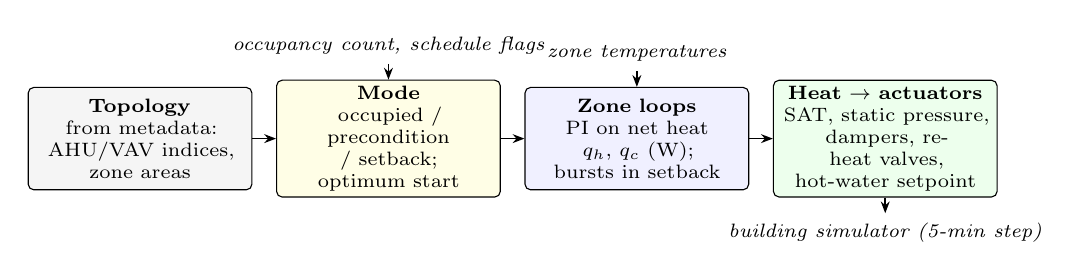
\begin{tikzpicture}[font=\scriptsize, node distance=3mm,
  box/.style={draw, rounded corners=2pt, align=center, inner sep=2pt, minimum height=13mm, text width=27mm},
  arr/.style={-{Stealth[length=1.5mm]}, semithick}]
\node[box, fill=gray!8] (topo) {\textbf{Topology}\\ from metadata:\\ AHU/VAV indices,\\ zone areas};
\node[box, fill=yellow!10, right=of topo] (mode) {\textbf{Mode}\\ occupied / precondition\\ / setback;\\ optimum start};
\node[box, fill=blue!6, right=of mode] (zone) {\textbf{Zone loops}\\ PI on net heat\\ $q_h$, $q_c$ (W);\\ bursts in setback};
\node[box, fill=green!7, right=of zone] (act) {\textbf{Heat $\to$ actuators}\\ SAT, static pressure,\\ dampers, reheat valves,\\ hot-water setpoint};
\draw[arr] (topo) -- (mode);
\draw[arr] (mode) -- (zone);
\draw[arr] (zone) -- (act);
\node[above=2mm of mode, font=\scriptsize\itshape] (occ) {occupancy count, schedule flags};
\draw[arr] (occ) -- (mode);
\node[above=2mm of zone, font=\scriptsize\itshape] (tz) {zone temperatures};
\draw[arr] (tz) -- (zone);
\node[below=2mm of act, font=\scriptsize\itshape] (b) {building simulator (5-min step)};
\draw[arr] (act) -- (b);
\end{tikzpicture}
\caption{One SADR control step. The topology is read once from the metadata; the mode, zone loops and actuator translation run every step. Every gain scales with the zone's floor area, so nothing depends on the size of the building.}
\label{fig:sadr}
\end{figure}

\paragraph{Topology from metadata.} Index tables come from the observation field names, the positional AHU action lists, the per-VAV action indices and the AHU-to-zone assignments; ranges and statistics come from the normalization metadata. Every action slot is written and clipped on every step. Nothing depends on the number of zones or handlers, the floor plan or the weather; non-finite inputs fall back to schedule values; there are no files, no network and no randomness.

\paragraph{Modes.} The controller is \textsc{Occupied} when the \texttt{comfort\_mode\_now} flag is set and the building is not detected as closed, in \textsc{Precondition} when unoccupied but comfort hours start within a lead time (or \texttt{comfort\_mode\_soon}), and in \textsc{Setback} otherwise. ``Somebody is here'' is detected relative to the running minimum of the affinely normalized occupancy count; a weekday on which nobody has arrived by \ParHolidayCheckH{}:00 is a holiday in the kit's occupancy model and is treated as unoccupied until the count rises. The optimum-start lead is $\ell = \ell_0 + \text{deficit}/(\hat{r}/s)$ ($\ell_0 = \RElvParLeadBaseH$\,h): the worst zone's distance from the comfort band over a recovery-rate estimate $\hat{r}$ (K/h), re-estimated from each morning's recovery (exponential average, weight \ParRateEma), with safety factor $s=\ParLeadSafety$, clipped to $[\ParLeadMinH, \ParLeadMaxH]$\,h. An online second-order zone model may shorten, but never lengthen, this lead.

\paragraph{Zone loops on net heat.} Each zone has heating and cooling targets: the sensor band shrunk by \ParMarginOcc\,K (occupied) or \ParMarginPre\,K (preconditioning). Two PI loops compute requested net heat $q_h = k_q (T_h^\star - T)^+ + I_h$ and cooling $q_c = k_q (T - T_c^\star)^+ + I_c$ in watts ($k_q = \ParKqWPerK$\,W/K, integral gain \ParKiWPerKStep\,W/K per step). The integrals unwind past the target, so a zone inside the band free-floats, and the larger request wins. The loops control net heat rather than flow because the zone-air node responds within minutes: a flow-proportional controller with a 5-minute step oscillates, whereas a net-heat gain of the order of the air node's conductance to the slab is stable, and the integral carries the steady load. In setback a running handler pays the ventilation load of every zone it serves, so the floor (the out-of-hours band of 289--298\,K widened by \ParNightLowExt{}/\ParNightHighExt\,K on weeknights, and by \RTenWkExtLo\,K more far from the next workday) is held by bursts: a zone that crosses it requests \ParQSbW\,W until it is \ParSbHystK\,K inside, and the handler is off otherwise. Holding the floor with the PI loops instead kept a handler running for \VthreeAhuOnUnocc{} of the unoccupied steps on the coldest scenario.

\paragraph{From heat to actuators.} A cooling zone needs capacity rate $F = q_c/(T - T_{\text{sa}})$, $T_{\text{sa}}$ being the AHU's estimated supply temperature; a heating zone is bounded by the discharge limit, $F = q_h/(308.15 - \delta - T)$, with a discharge margin $\delta = \ParDischMarginK$\,K. A cooling handler commands the coldest supply air (SAT), \ParSatCoolHi\,K. The coil load is $q_c + F\,(T_{\text{mixed}} - T)$ at a constant COP, so the ventilation term and fan power fall with flow; a Guideline~36 upward reset~\citep{ashrae2021g36,taylor2018vav} is right in a real building but wrong here. A handler that also heats is floored at \ParSatMixFloor\,K, so its cooling zones are not overcooled into reheat, and a heating-only handler commands 305\,K, so the coil idles. Static pressure is trim-and-respond in closed form, $P = P_{\text{design}}\max_z f_z^2$ clipped to $[200, 2000]$\,Pa with $f_z$ each zone's requested fraction of design flow, so the most demanding damper is fully open; dampers are $f_z/\sqrt{P/P_{\text{design}}}$. Occupied flow above the 200\,Pa floor is granted only in proportion to the zone's error.

\paragraph{Reheat, on/off and hot water.} The discharge temperature that delivers $q_h$ at the delivered flow gives the water capacity rate $W_z = F_z\,(T_{\text{disch}} - T_{\text{sa}})/(T_w - T_{\text{sa}})$. The loop differential pressure is reset so the largest $W_z$ sits at \ParValveTarget{} of valve travel, and each valve is $W_z/(k_v \sqrt{\Delta p})$, $k_v$ being the valve's flow coefficient at full opening. An AHU runs iff a served zone requests more than $q_{\text{on}} = \RElvParQOnW$\,W (dwell \ParMinOnSteps{} steps), and the pump runs iff a valve is open. Recirculation is at the 0.7 cap, except when a cooling-only handler sees outside air colder than return air by more than the exhaust-fan break-even ($0.00322\,\text{K/Pa}\times P$); the outside-air fraction is then solved so the mixed air lands on the SAT target, and outside heating season a night flush uses outside air at least \ParRFFlushDt\,K colder. In heating season the forced minimum air of set-back zones on a running handler is reheated, which buys heat at 1\,J of gas per joule. The hot-water setpoint is 350\,K during a heating season (heating requested within the last \RTenSeasonSteps{} steps while the outside air fell below \RTenSeasonOatC\,$^\circ$C within a day) and 310\,K otherwise. Gas is billed as heat delivered, so hotter water costs only a tank dissipation of \TankLossExtraKw\,kW while widening the coils' reach; in the ablation (Table~\ref{tab:ablation12}) 330\,K instead changes the public loss by \RElvAbTwRel.

\paragraph{Scaling with the building.} Every zone's gains, request cap, setback burst and optimum start scale with its floor area, read from the metadata zone map (clipped to $[\ParAreaScaleMin, \ParAreaScaleMax]\times$ a \ParAreaRef\,m$^2$ zone), and each request is bounded by what the box and its coil can deliver, up to \RFiveParQcapKw\,kW per 100\,m$^2$. The day of week is rounded after decoding, because float32 sine and cosine decode Saturday as 4.999999999, which a test ``day $<5$'' counts as a workday.

\paragraph{Development protocol.} The controller just described, which we call the \emph{base} controller and analyse in Sections~\ref{sec:results} and~\ref{sec:analysis}, took ten rounds (Table~\ref{tab:rounds}, Appendix~\ref{app:rounds}). The first two chose constants on the public set, by a seeded random search over \NTuneConfigs{} configurations and then \NCandV{} physics-motivated candidates. From the third round on, single changes were screened on public and generated scenarios, the helpful ones combined, and the result shipped only under a rule written down before its confirmation runs: not worse on the public set, and better at full length on scenarios not used to choose it. As hidden-leaderboard feedback arrived (Section~\ref{sec:results}), the confirmation sets moved from generated buildings under public weather to harsh weather and finally to harsh weather on new buildings. Two later steps (Section~\ref{sec:tuning}) tuned the base controller's constants and added one structural change, giving the \emph{final} controller.

\section{Results}
\label{sec:results}

\paragraph{Setup.} All runs use the kit's environment loader and \texttt{SimulationTracker}, 8,640 steps per scenario, and the kit's leaderboard formula, with paired bootstrap 95\% CIs over scenarios. Besides the 30 public scenarios (six shipped buildings $\times$ five stations), we report a \emph{cold} set of \RTenConfHarshCThreeN{} and a \emph{hot} set of \RTenConfHotHN{} harsh 30-day strips on \RTenNNewBuild{} new buildings from the shipped generator ranges, and a \emph{harsh screening} set of \RSixHarshSN{} cold scenarios on the shipped buildings; Appendix~\ref{app:rounds} lists the earlier sets. Seeds are fixed and runs reproduce across machines (SADR bit for bit on a laptop and on Kaggle in \RSixReproIdentical{} of \RSixReproN{} checks). Local \texttt{pid\_water} returns differ from the shipped \texttt{baseline\_returns.json} by $\GapMeanPidWater$ on average and by $\GapMinPidWater$ to $\GapMaxPidWater$ per scenario, so all comparisons use local runs.

% Built by hand on 2026-11-14 from table_main_r11.tex (generated by make_macros_r11.py) plus the tuned and final
% rows (sources in results_macros_final.tex). Ratios are to the base controller.
\begin{table}[t]
\caption{Leaderboard metric on the 30 public scenarios (mean over scenarios of $|$mean per-step reward$|$; lower is better) and per-station means. Ratio: mean of the row over the mean of the base controller, with a paired bootstrap 95\% CI over scenarios; wins: scenarios where the base controller is beaten by an SADR row, or beats a baseline. The last row uses the organizers' shipped returns instead of local runs. Every development version is in Table~\ref{tab:versions}.}
\label{tab:main}
\centering\scriptsize
\setlength{\tabcolsep}{3pt}
\begin{tabular}{lcccccccc}
\toprule
policy & all & Fairbanks & Denver & Atlanta & Phoenix & Singapore & ratio [95\% CI] & wins \\
\midrule
SADR, final (tuned + ramp) & \textbf{0.00730} & 0.01460 & 0.00414 & 0.00484 & 0.00714 & 0.00580 & 0.980 [0.966, 0.989] & 27/30 \\
SADR, tuned constants & 0.00733 & 0.01461 & 0.00417 & 0.00489 & 0.00715 & 0.00584 & 0.983 [0.972, 0.990] & 27/30 \\
SADR, base (analysed) & 0.00745 & 0.01475 & 0.00440 & 0.00498 & 0.00726 & 0.00588 & 1 & -- \\
\midrule
\texttt{pid\_water} & 0.05498 & 0.07908 & 0.03794 & 0.03064 & 0.08009 & 0.04714 & 7.37 [6.02, 9.29] & 30/30 \\
\texttt{fixed\_setpoint} & 0.06550 & 0.07586 & 0.07721 & 0.03296 & 0.11615 & 0.02533 & 8.79 [6.31, 12.29] & 30/30 \\
\texttt{bang\_bang} & 0.22453 & 0.19959 & 0.18300 & 0.23151 & 0.23673 & 0.27183 & 30.12 [21.39, 42.19] & 30/30 \\
\texttt{pid\_water} (organizer values) & 0.05414 & 0.07847 & 0.03735 & 0.03010 & 0.07814 & 0.04665 & 7.26 [5.93, 9.13] & 30/30 \\
\bottomrule
\end{tabular}
\end{table}


\paragraph{Main result.} The final controller reaches \FinPub{} on the public set and the base controller \RTenConfPubCand, against \MetricPidWater{} for \texttt{pid\_water} (Table~\ref{tab:main}). The base controller's loss is \RElvPwTimes{} times lower (ratio \RElvPwRatio, paired 95\% CI \RElvPwRatioLo--\RElvPwRatioHi; resampling the six buildings instead, \RElvPwRatioCLo--\RElvPwRatioCHi) and lower on \RElvPwWins{} scenarios; tuning and the structural change remove a further \(2.0\%\) (ratio \FinPubRatio, CI \FinPubRatioLo--\FinPubRatioHi, lower on \FinPubWins). The gains shrank as the controller matured, from \CandWinnerRelRed{} in the second round to \RTenConfPubRelAbs{} in the tenth, and one round shipped nothing. Scenarios share buildings and stations, so the scenario bootstrap understates the width of the intervals, though not their sign.

\paragraph{Transfer to unseen buildings.} Because nothing in SADR is fitted to a building, the main risk is buildings unlike the public six. On \NHeldAll{} scenarios of \NHeldAllBuild{} generated buildings drawn from the kit's wider default ranges, the first area-scaled version scored \HeldAllMetricOurs{} against \HeldAllMetricPidWater{} for \texttt{pid\_water} (Figure~\ref{fig:heldout}), and every later change was confirmed on buildings or weather that had not selected it.

\paragraph{What each mechanism is worth.} Table~\ref{tab:ablation12} removes one mechanism at a time from the base controller and runs the public set at full length; the reference runs reproduce the development runs \RElvAbRefMatch. One mechanism carries most of the margin. Replacing the coldest supply air with an upward reset raises the loss by \RElvAbSatRel, all of it in energy cost and carbon (comfort improves slightly), and the effect is concentrated in a few scenarios. Scaling every zone's gains with its floor area is the most consistent mechanism (\RElvAbNoareaRel, lower on all 30 scenarios), and five more are each worth about one per cent: the deeper weekend setback (\RElvAbNoweekendRel), the cap on requests at what the coil can deliver (\RElvAbNowcapRel, binding on only three scenarios), rounding the decoded day of week (\RElvAbNodowRel), per-zone optimum start (\RElvAbNozoneRel) and reheating set-back forced air (\RElvAbNoneutralRel). The economizer, the set-back air boost, the model-based start and the heating season add under one per cent each. Four mechanisms are inert on the public set: the 350\,K hot water (\RElvAbTwRel), the recoverable setback floor (\RElvAbNofloorRel), the night flush (\RElvAbNoflushRel) and error-proportional occupied flow (\RElvAbNooccdynRel). Each entered as part of a bundle and none was confirmed alone, so the public ablation cannot show whether they help in colder hidden weather.

% table_ablation_r11.tex (generated by make_macros_r11.py) with version tags removed by hand, 2026-11-14
\begin{table}[t]
\caption{Leave-one-out ablation of the base controller on the 30 public scenarios (8,640 steps). Each row changes one mechanism and keeps the rest of the base controller. Change: mean loss of the arm against the base controller (\RElvAbRefLoss), paired bootstrap 95\% CI over scenarios and over the six buildings (cluster); positive = the mechanism helps. Wins/losses: scenarios where the base controller is lower/higher. Terms: change in comfort, energy cost and carbon as a share of the base controller's loss. The arms were fixed before any run.}
\label{tab:ablation12}
\centering\scriptsize
\setlength{\tabcolsep}{2pt}
\begin{tabular}{>{\raggedright\arraybackslash}p{3.8cm}cccc>{\raggedright\arraybackslash}p{2.5cm}}
\toprule
mechanism removed (arm) & loss & change [95\% CI] & cluster CI & wins/losses & comfort, energy, carbon \\
\midrule
zone gains scaled with zone area & 0.00762 & $+$2.2\% [$+$1.6\%, $+$3.2\%] & [$+$1.5\%, $+$3.5\%] & 30/0 & $+$2.0\%, $+$0.1\%, $+$0.1\% \\
per-zone optimum start & 0.00754 & $+$1.1\% [$+$0.3\%, $+$2.0\%] & [$+$0.5\%, $+$1.9\%] & 17/13 & $-$0.8\%, $+$0.6\%, $+$1.4\% \\
setback floor limited to what the zone recovers & 0.00745 & $+$0.0\% [$-$0.1\%, $+$0.0\%] & [$-$0.1\%, $+$0.0\%] & 3/19 & $+$0.0\%, $+$0.0\%, $+$0.0\% \\
requests capped at the coil's delivery & 0.00755 & $+$1.3\% [$+$0.0\%, $+$3.0\%] & [$+$0.0\%, $+$2.8\%] & 3/0 & $+$0.5\%, $+$0.4\%, $+$0.4\% \\
economizer & 0.00751 & $+$0.8\% [$+$0.3\%, $+$1.5\%] & [$+$0.4\%, $+$1.5\%] & 26/2 & $+$0.0\%, $+$0.6\%, $+$0.1\% \\
coldest supply air (arm: upward reset, ceiling 293\,K) & 0.00801 & $+$7.4\% [$+$2.7\%, $+$13.5\%] & [$+$5.8\%, $+$9.1\%] & 15/13 & $-$0.7\%, $+$6.9\%, $+$1.3\% \\
350\,K hot water in heating season (arm: 330\,K) & 0.00745 & $+$0.0\% [$-$0.6\%, $+$0.4\%] & [$-$0.5\%, $+$0.3\%] & 4/26 & $+$0.2\%, $+$0.1\%, $-$0.3\% \\
occupied flow in proportion to the error & 0.00747 & $+$0.2\% [$+$0.0\%, $+$0.3\%] & [$+$0.0\%, $+$0.3\%] & 15/1 & $-$0.4\%, $+$0.2\%, $+$0.3\% \\
night flush & 0.00746 & $+$0.1\% [$+$0.0\%, $+$0.3\%] & [$+$0.1\%, $+$0.2\%] & 13/3 & $+$0.0\%, $+$0.2\%, $+$0.0\% \\
set-back forced air reheated to zone temperature & 0.00753 & $+$1.1\% [$+$0.0\%, $+$1.8\%] & [$+$0.3\%, $+$1.6\%] & 8/12 & $+$0.2\%, $+$0.3\%, $+$0.6\% \\
deeper weekend setback & 0.00755 & $+$1.3\% [$+$0.3\%, $+$2.1\%] & [$+$0.4\%, $+$2.0\%] & 19/1 & $+$0.0\%, $+$0.5\%, $+$0.8\% \\
request cap 20\,kW per 100\,m$^2$ (arm: 12\,kW) & 0.00748 & $+$0.3\% [$+$0.0\%, $+$0.8\%] & [$+$0.0\%, $+$0.8\%] & 4/4 & $+$0.4\%, $+$0.0\%, $+$0.0\% \\
set-back air boost & 0.00751 & $+$0.7\% [$+$0.1\%, $+$1.2\%] & [$+$0.2\%, $+$1.0\%] & 12/5 & $+$0.1\%, $+$0.2\%, $+$0.4\% \\
model-based starts & 0.00752 & $+$0.8\% [$+$0.4\%, $+$1.5\%] & [$+$0.4\%, $+$1.4\%] & 18/1 & $-$0.4\%, $+$0.4\%, $+$0.8\% \\
day of week rounded after decoding & 0.00755 & $+$1.2\% [$+$0.9\%, $+$1.6\%] & [$+$0.9\%, $+$1.7\%] & 29/1 & $+$0.0\%, $+$0.5\%, $+$0.8\% \\
7-day heating season below 15\,$^\circ$C & 0.00751 & $+$0.8\% [$+$0.5\%, $+$1.1\%] & [$+$0.6\%, $+$1.0\%] & 18/1 & $+$0.0\%, $+$0.2\%, $+$0.6\% \\
\bottomrule
\end{tabular}
\end{table}


\paragraph{What the hidden leaderboard indicates.} Kaggle's public leaderboard scores about ten of the 30 hidden scenarios: six new buildings from the same generator under five stations absent from the public set. An early version scored \RFiveKagGapPub{} times its public-set number there, although Kaggle reproduces a public scenario's local total to 0.02\%. Submitting several versions and \texttt{pid\_water} separated buildings from weather (Table~\ref{tab:kaggle}, Appendix~\ref{app:rounds}). Ratios between our versions on Kaggle matched those on the public set rather than on larger generated buildings, which suggests that the hidden buildings behave like the shipped six; \texttt{pid\_water}'s ratio was lower on Kaggle than on the public set, as colder hidden weather would predict. A mixture of \RSixMixWPct{} harsh and the rest public scenarios, fitted to one version's Kaggle score, predicts \texttt{pid\_water}'s Kaggle ratio (\RSixMixPid{} against \RSixKagRatioPid), which is why later rounds confirmed on harsh weather. The final controller scores \RFtKagVFourteen{} (rank \FinKagRank{} of \FinKagTeams{} teams on 14 November; best entry \FinKagBest, median \FinKagMedian). These readings rest on about ten hidden scenarios and one submission per version.

\subsection{Tuning the constants}
\label{sec:tuning}

\paragraph{Protocol.} The base controller's constants were set from physics and single-change screens and never searched jointly. We searched \RTwNParams{} of them at once (setback depths and burst heat, the set-back air boost, optimum-start lead and safety, comfort margins, PI gains, valve target and mixed-air floor; Table~\ref{tab:params13}) with CMA-ES~\citep{hansen2016cma}: population \RTwPop, \RTwGens{} generations, initial step size \RTwSigmaZero{} in the box scaled to $[0,1]$, started at the base values. The objective was the loss ratio to the base on \RTwWinDays-day windows of \RTwNWin{} fixed scenarios, weighted a third on \RTwNWinHarsh{} harsh scenarios and two thirds on \RTwNWinPub{} public-like ones, the mixture that matched the hidden leaderboard. The plan, hashed before any run, kept the setback depths within \RTwDepthMaxDeeper\,K of the base values, fixed the candidate as the final CMA mean rather than the best sample, and fixed the rule: at full length the 95\% CI of the mixture ratio ($\tfrac13$\,cold $+$ $\tfrac23$\,hot) must lie below one, and the public set must not be worse. The cold and hot sets had already selected the base controller, so reusing them favours it. The median candidate's window ratio fell from \RTwMedFirst{} in the first generation to \RTwMedLast{} in the last, and the CMA mean passed the rule: mixture \RTwCandMix{} (CI \RTwCandMixLo{} to \RTwCandMixHi), public \RTwCandPub{} (Table~\ref{tab:tuning13}).

\paragraph{Black-box search finds the missing frost cost.} The plan also required the frost exposure on the harsh screening set to be reported, and part of the gain came from there. The search had moved both weeknight setback depths towards their bounds (floor widening \RTwCandNightLow{} against the base \RTwVTwelveNightLow\,K, ceiling \RTwCandNightHigh{} against \RTwVTwelveNightHigh\,K); its coldest zone reached \RTwCandColdest\,$^\circ$C against the base controller's \RTwVTwelveColdest\,$^\circ$C, and its share of zone-steps below 5\,$^\circ$C rose by \RTwCandBelowFiveRise{} points. Restoring the base depths while keeping the other twelve tuned constants keeps the public gain (\RTwVarPub) and about half of the mixture gain (\RTwVarMix, CI \RTwVarMixLo{} to \RTwVarMixHi), at the base controller's below-5\,$^\circ$C share and a coldest zone \RTwVarColderK\,K colder. A second search asked whether a re-tune with the depths held fixed recovers the rest. Its plan, hashed before its runs, added a frost guard (below-5\,$^\circ$C share at most \RTwGuardPP{} points above the base, coldest zone at most \RTwGuardK\,K below it) and a mechanical choice among the candidates that pass every rule. The re-tune (\RTwNParamsThr{} constants, \RTwGensThr{} generations) recovered the whole mixture gain (\RTwThrMix, CI \RTwThrMixLo{} to \RTwThrMixHi) and the frost exposure with it: coldest zone \RTwThrColdest\,$^\circ$C, below-5\,$^\circ$C share \RTwThrBelowFiveRise{} points above the base. With the depths closed, the search reached cold buildings through the heat that defends them, cutting the setback burst from \RTwVarQSb{} to \RTwThrQSb\,W and the base preconditioning lead from \RTwVarLeadBase{} to \RTwThrLeadBase\,h. We read this as a general hazard: a reward that charges nothing for an empty building far below freezing is optimised towards one by whichever constants remain free, so a physical constraint absent from the reward has to enter the selection rule.

\paragraph{The tuned controller.} The rule ships the restored-depth candidate: a modest gain whose interval excludes zero (\RTwVarHCThree{} on the cold set, \RTwVarHH{} on the hot set, \RTwVarPub{} on the public set) at the base controller's frost exposure, scoring \RTwKagVThirteen{} on Kaggle against \RTenKagVTwelve{} for the base. The evidence is weaker than for the base controller: the candidate was constructed after the first search's frost result, the frost guard was written when its interim frost numbers were known, and the frost measurements include the scenarios whose windows were tuned on. The two rejected candidates stay in Table~\ref{tab:tuning13} as sensitivity results; they indicate what this reward pays for colder set-back buildings, about \RTwCandMixAbs{} on the mixture against \RTwVarMixAbs{} for the frost-neutral tune.

\paragraph{A structural change: the cooling handover ramp.} Tuning leaves the structure untouched, so a last round screened \RFtNScreen{} structural switches on top of the tuned controller, each off by default (all off reproduces it bit for bit). One passed its screen and its confirmation: a zone's occupied cooling target starts at its preconditioning target and moves to the occupied one over the first occupied hour. Without it, a zone that arrives warm at the end of its morning recovery overshoots the band in the first occupied steps. At full length, under a plan hashed before the runs, the ramp lowers the mixture loss by \RFtMixAbs{} (CI \RFtMixLo{} to \RFtMixHi), almost all of it on the hot set (\RFtHH, lower on \RFtHHWins{} scenarios, where it cuts comfort regret by \RFtHHRegretCut; cold set \RFtHCThree), and the public loss by \RFtPubAbs{} (\RFtPubWins). It does not touch the setback, and its frost exposure equals the tuned controller's (coldest zone \RFtColdest\,$^\circ$C, \RFtBelowFive{} of zone-steps below 5\,$^\circ$C). It is the final controller, and scores \RFtKagVFourteen{} on Kaggle against \RTwKagVThirteen{} without it.

% table_tuning_r12.tex (generated by make_macros_r12.py) with descriptive row names, by hand, 2026-11-14
\begin{table}[t]
\caption{Tuning the constants: full-length confirmation against the base controller. Free search: the CMA mean over all \RTwNParams{} constants; re-tuned: a second search with the setback depths fixed at the base values; tuned (shipped): the free search's constants with the base setback depths restored. Depths: weeknight floor/ceiling widening in K. Mixture: the pre-registered $\tfrac13$\,cold $+$ $\tfrac23$\,hot mean ratio to the base minus one, with its paired bootstrap 95\% CI (stratified by set); cold, hot and public: mean change of the loss (wins). Harsh (\RTwNHS{} harsh screening scenarios with time series): loss change, coldest zone temperature ($^\circ$C) and share of zone-steps below 5\,$^\circ$C. Guard: the frost guard (fixed in the second search's plan): below-5\,$^\circ$C share at most \RTwGuardBelowFiveLim{} and coldest zone at least \RTwGuardColdestLim\,$^\circ$C. All three candidates pass the primary rule and the public guard; only the shipped tuned controller passes the frost guard.}
\label{tab:tuning13}
\centering\scriptsize
\setlength{\tabcolsep}{1.5pt}
\begin{tabular}{@{}llcccccccc@{}}
\toprule
controller & depths & mixture [95\% CI] & cold & hot & public & harsh & coldest & $<$5\,$^\circ$C & guard \\
\midrule
base & 10.0/6.0 & -- & -- & -- & -- & -- & $-$9.4 & 4.24\% & -- \\
free search & 11.5/7.9 & $-$0.74\% [$-$0.98\%, $-$0.50\%] & $-$1.01\% (39/40) & $-$0.60\% (28/40) & $-$2.6\% (28/30) & $-$1.0\% & $-$11.4 & 4.89\% & fail \\
re-tuned & 10.0/6.0 & $-$0.74\% [$-$0.93\%, $-$0.54\%] & $-$0.70\% (34/40) & $-$0.76\% (34/40) & $-$3.0\% (29/30) & $-$0.8\% & $-$11.0 & 4.66\% & fail \\
\textbf{tuned (shipped)} & 10.0/6.0 & $-$0.39\% [$-$0.65\%, $-$0.12\%] & $-$0.68\% (36/40) & $-$0.24\% (21/40) & $-$2.5\% (27/30) & $-$0.8\% & $-$10.0 & 4.24\% & pass \\
\bottomrule
\end{tabular}
\end{table}


\section{Analysis}
\label{sec:analysis}

\begin{figure}[t]
\centering
\figfile{0.92\linewidth}{figures/fig_loss_by_hour_v12.pdf}
\caption{Mean loss per step by hour of day over the 30 public scenarios, split into comfort regret and energy\,+\,carbon (comfort hours 06--19 shaded; note the different scales). Left: SADR (base); right: \texttt{pid\_water}.}
\label{fig:hours12}
\end{figure}

\paragraph{Why it wins, and where the loss sits.} The two controllers lose in different places (Figure~\ref{fig:hours12}). \texttt{pid\_water}'s loss is mostly comfort regret in occupied hours: with one loop per handler and a step start at 06:00, it keeps \OccOutPidWater{} of occupied zone-steps outside the band. SADR's loss is energy, and its largest hourly loss falls at hour \RElvHourPeak{}, the end of the morning warm-up; \RElvUnoccHourShare{} of it falls outside 06:00--19:00. Its energy use stays low through floor pressure with wide dampers, the least reheat flow at the discharge cap, and no conditioning while nobody is charged for comfort. Fairbanks is gas (Eq.~\ref{eq:g}); Phoenix and Singapore are chiller electricity, where the coldest supply at the lowest flow is cheapest.

\paragraph{Where the gas goes in harsh weather.} On the harsh screening set, a mid-development version pays \RSixDecGas{} of its loss for gas: \RSixDecOccWd{} of it in occupied weekday hours, \RSixDecPreWd{} in weekday preconditioning, \RSixDecPreWe{} in weekend preconditioning and \RSixDecSbWe{} in weekend setback. The outside-air load of running handlers equals a fraction \RSixDecVent{} of the gas, \RSixDecVentHeated{} of it through zones being heated.

\paragraph{What each heating lever is worth.}
From the kit's equations, a box delivers the net heat $Q=\rho c_p F (T_d - T)$ while its coil, which the boiler bills, supplies $\rho c_p F (T_d - T_{sa})$, with $T_{sa}=\min(\text{SAT}, r\,T_{\text{ret}} + (1-r)\,T_{\text{out}})$ and $r\le 0.7$. One joule of net heat therefore costs
\begin{equation}
g = \frac{T_d - T_{sa}}{T_d - T} = 1 + \frac{T - T_{sa}}{T_d - T}
\label{eq:g}
\end{equation}
joules of coil duty, which holds in the simulator to within \RSevGErr{} (the kit's methods wrapped); billed gas is \RSevGasOverCoil{} times the coil duty.
Two of these levers are already spent. In a check on building~8 in January, the handlers sit at the recirculation cap on \RSevRecircCapShare{} of their steps, and \RSevCapHeatShare{} of the net heat enters at the 308.15\,K discharge cap. For a zone at 21$^\circ$C, $g$ is \RSevGZero{} at 0$^\circ$C outside and \RSevGMinusForty{} at $-40^\circ$C (\RSevGColdZero{} and \RSevGColdMinusForty{} for a zone at 8$^\circ$C). What control still chooses is when, and at which zone temperature, heat goes in. Fitted on \RSevNZones{} zones of six harsh scenarios, a first-order model $\dot T = aQ - k(T - T_{\text{out}}) + c$ has a median time constant of \RSevTauMed\,h (\RSevTauLo--\RSevTauHi\,h), explains only \RSevRTwo{} of the 30-minute variance (median) and predicts a recovery's duration with a median error of \RSevRecErr. At the cap, the recovery rate falls by \RSevRateSlope\,K/h for each K the zone is warmer.

In this model a deeper setback floor never costs gas if the zone reaches it and recovers in time (its trajectory lies below the shallower one, and both the losses and $g$ grow with $T$). Depth pays only where the floor binds, on \RSevBindLo--\RSevBindHi{} of unoccupied zone periods in a mid-development version. With capped heat the latest feasible start is optimal, so a start rule can save at most the time zones hold at the target before 06:00: \RSevHoldH\,h per recovery, \RSevHoldGas{} of the gas. Twelve seven-day checks on three harsh scenarios test these predictions (Table~\ref{tab:checks_r7}). Floor predictions hold within 0.5 points in buildings~7 and~8 and fail in building~1, whose zones cool slowest: a 2\,K deeper floor changes the gas by $\RSevChkEightNleMeas$ (predicted $\RSevChkEightNlePred$) in building~8, where the floor binds most, but by $\RSevChkOneNleMeas$ (predicted $\RSevChkOneNlePred$) in building~1. Start-time predictions overstate the saving in buildings~8 and~1; in building~7 a lead safety of 1.0 changes the gas by $\RSevChkSevenLsOMeas$ (predicted $\RSevChkSevenLsOPred$) but the loss only by $\RSevChkSevenLsOLoss$, because part returns as comfort.

\paragraph{Pitfalls in the kit.} Two details of the kit affect any controller. The decoded day of week has to be rounded: float32 sine and cosine put Saturday at 4.999999999, so a test ``day $<5$'' makes it a workday, and in our development runs the resulting Saturday-morning recovery carried a large share of the cold-weather loss (Appendix~\ref{app:note-v11}). The shipped baseline returns differ from local runs by up to $\GapMinPidWater$ per scenario, so comparisons should use local runs.

\section{Limitations and disclosure}
\label{sec:limits}
\paragraph{Deep cold.} SADR loses most in deep cold: the base controller's worst public scenario, \RElvWorstPubScen, scores \RElvWorstPub, \RElvWorstPubComfortShare{} of it comfort and the rest almost all gas.

\paragraph{Simulator gaps.} SADR does not use the boiler-billing gap that starter-kit pull request~\#2 closes. In a patched kit an early SADR's loss falls by \RFivePrTwoVSevenRelAbs{} on the \RFivePrTwoVSevenN{} public Fairbanks scenarios while \texttt{pid\_water}'s rises by \RFivePrTwoPidRelAbs, and SADR leaves out a hot-water ramp whose saving came only from that gap (Appendix~\ref{app:note-v11}). We treat a billing error the organizers have a fix for as out of bounds and take the reward as written otherwise. The reward has no frost cost, and SADR's weekend setback uses that: on the harsh screening set the base controller's coldest zone reaches $\RElvColdestHS^\circ$C (\RElvBelowFiveHS{} of zone-steps below 5$^\circ$C), and a 5$^\circ$C frost floor would cost it \RElvFrostHsRel{} there (95\% CI \RElvFrostHsLo{} to \RElvFrostHsHi). Black-box tuning exploits the same gap (Section~\ref{sec:tuning}), so further tuning against this simulator needs a frost guard or a frost term in its objective. A real deployment needs that floor, and it would also commission the simulator constants SADR encodes (discharge limit, valve $k_v$, constant COP).

\paragraph{Unconfirmed parts.} Each Kaggle score rests on about ten hidden scenarios and one submission. The tuned controller's confirmation reused sets that had already selected the base controller, and its frost guard was fixed after its interim frost numbers were known. The \RTenSeasonOatC\,$^\circ$C heating-season gate is supported only by development runs, because the cold confirmation windows never exercise it. The last structural round of the base controller lowered energy and carbon by accepting \RTenComfRiseHCThree{} more comfort regret on the cold set (\RTenComfRisePub{} on the public set), and on larger default-range generated buildings, outside every confirmation rule, the late refinements shrink or vanish.

\paragraph{Selection.} Selection used the public set and screens, so the public number is optimistic; the confirmations estimate the size of each change (Table~\ref{tab:rounds}), and Kaggle estimates the level.

\paragraph{Next step.} The best Kaggle entries score \FinKagBest, less than half of the final controller's loss, so much of the remaining gain is reachable. A natural next step is a model-predictive controller on the kit's own linear building model, or a learned residual on top of SADR that keeps its structure. A perfect-foresight linear programme on that model saves \RElvLpMin--\RElvLpMax{} (mean \RElvLpMean) of an intermediate version's loss on \RElvLpN{} heating scenarios (Appendix~\ref{app:note-v11}), mostly in holding the weekend floor and in timing weeknight recovery; how much of that is reachable without foresight is open.

\paragraph{Reproducibility and disclosure.} \texttt{experiments/src/} and \texttt{paper/make\_macros\_*.py} generate the numbers in the text and the generated tables (seeds fixed, CPU only), and \texttt{paper/AUDIT.md} checks each against its source file. We used Claude (Anthropic) as an AI assistant. Code and policy: \url{https://github.com/neelsirivara/neurips2026-smart-buildings}.
\bibliographystyle{plainnat}
\bibliography{refs}

\clearpage
\appendix
\paragraph{Version numbers.} The appendix keeps the development record, where versions are numbered as they shipped: the base controller of the main text is v12, the tuned controller v13 and the final controller (with the cooling handover ramp) v14. Set codes: P is the public set, HC3 the cold set, HH the hot set and HS the harsh screening set of Section~\ref{sec:results}; the remaining codes are defined in Table~\ref{tab:rounds}.
\section{Per-scenario results}
\label{app:per_scenario}
% generated by paper/make_macros_r11.py; do not edit
\begin{table}[!htbp]
\caption{Every SADR version on the public scenarios, as Table~\ref{tab:main}. Machines: v12 and v9 the M5 Pro, v11 and v10 Kaggle CPU kernels, v8 and earlier the laptop; SADR reproduces bit for bit on laptop and Kaggle and within \RSixMacReproMaxRel{} on the M5 Pro.}
\label{tab:versions}
\centering\scriptsize
\setlength{\tabcolsep}{3pt}
\begin{tabular}{lcccccccc}
\toprule
policy & all & Fairbanks & Denver & Atlanta & Phoenix & Singapore & ratio to v12 [95\% CI] & v12 wins \\
\midrule
SADR v12 (shipped) & \textbf{0.00745} & 0.01475 & 0.00440 & 0.00498 & 0.00726 & 0.00588 & 1 & -- \\
SADR v11 & 0.00753 & 0.01492 & 0.00449 & 0.00507 & 0.00729 & 0.00588 & 1.01 [1.01, 1.01] & 21/30 \\
SADR v10 & 0.00762 & 0.01516 & 0.00456 & 0.00512 & 0.00733 & 0.00593 & 1.02 [1.02, 1.03] & 28/30 \\
SADR v9 & 0.00775 & 0.01531 & 0.00467 & 0.00525 & 0.00741 & 0.00610 & 1.04 [1.03, 1.05] & 30/30 \\
SADR v8 & 0.00777 & 0.01561 & 0.00470 & 0.00523 & 0.00737 & 0.00593 & 1.04 [1.03, 1.06] & 30/30 \\
SADR v7 & 0.00786 & 0.01598 & 0.00471 & 0.00524 & 0.00741 & 0.00593 & 1.05 [1.03, 1.07] & 29/30 \\
SADR v6 & 0.00803 & 0.01673 & 0.00475 & 0.00530 & 0.00742 & 0.00594 & 1.08 [1.04, 1.10] & 29/30 \\
SADR v5 & 0.00831 & 0.01752 & 0.00497 & 0.00549 & 0.00755 & 0.00602 & 1.11 [1.07, 1.15] & 29/30 \\
\texttt{pid\_water} & 0.05498 & 0.07908 & 0.03794 & 0.03064 & 0.08009 & 0.04714 & 7.37 [6.02, 9.29] & 30/30 \\
\texttt{fixed\_setpoint} & 0.06550 & 0.07586 & 0.07721 & 0.03296 & 0.11615 & 0.02533 & 8.79 [6.31, 12.29] & 30/30 \\
\texttt{bang\_bang} & 0.22453 & 0.19959 & 0.18300 & 0.23151 & 0.23673 & 0.27183 & 30.12 [21.39, 42.19] & 30/30 \\
\texttt{pid\_water} (organizer values) & 0.05414 & 0.07847 & 0.03735 & 0.03010 & 0.07814 & 0.04665 & 7.26 [5.93, 9.13] & 30/30 \\
\bottomrule
\end{tabular}
\end{table}

Table~\ref{tab:versions} gives every SADR version on the public scenarios. Tables~\ref{tab:per_scenario}, \ref{tab:per_scenario_held} and~\ref{tab:per_scenario_held_r3}
list every scenario's total return and leaderboard score (SADR v6), and
Table~\ref{tab:per_scenario_fresh} the round-4 confirmation set, Table~\ref{tab:r4} round 4 at full length and
Table~\ref{tab:per_scenario_r5m} the round-5 Minneapolis set; all values are generated from the
result files by \texttt{make\_macros.py}.
\begin{table}[H]
\caption{Round 4 at full length (8,640 steps): the composite v7 against the shipped
v6 on the same scenarios; $\Delta$ = paired mean difference in $10^{-5}$ per step with its
bootstrap 95\% CI (\NBoot{} resamples; negative favours v7). Old clean = the round-2/3 held-out
scenarios no screen touched; fresh = \RFFreshNBuild{} buildings generated for round 4 and run only
for this table, half in the shipped six's parameter ranges, half in the kit's default ranges.}
\label{tab:r4}
\centering\scriptsize
\setlength{\tabcolsep}{4pt}
\begin{tabular}{lrrrrrr}
\toprule
set & $n$ & v6 & v7 & $\Delta$ [95\% CI] & relative [95\% CI] & wins \\
\midrule
public & \RFConfPubN & \RFConfPubVSix & \RFConfPubCand & \RFConfPubDiff{} [\RFConfPubLo, \RFConfPubHi] & \RFConfPubRel{} [\RFConfPubRelLo, \RFConfPubRelHi] & \RFConfPubWins \\
old held-out, clean & \RFConfOldCleanN & \RFConfOldCleanVSix & \RFConfOldCleanCand & \RFConfOldCleanDiff{} [\RFConfOldCleanLo, \RFConfOldCleanHi] & \RFConfOldCleanRel{} [\RFConfOldCleanRelLo, \RFConfOldCleanRelHi] & \RFConfOldCleanWins \\
fresh, shipped ranges & \RFConfFreshShipN & \RFConfFreshShipVSix & \RFConfFreshShipCand & \RFConfFreshShipDiff{} [\RFConfFreshShipLo, \RFConfFreshShipHi] & \RFConfFreshShipRel{} [\RFConfFreshShipRelLo, \RFConfFreshShipRelHi] & \RFConfFreshShipWins \\
fresh, default ranges & \RFConfFreshDefN & \RFConfFreshDefVSix & \RFConfFreshDefCand & \RFConfFreshDefDiff{} [\RFConfFreshDefLo, \RFConfFreshDefHi] & \RFConfFreshDefRel{} [\RFConfFreshDefRelLo, \RFConfFreshDefRelHi] & \RFConfFreshDefWins \\
fresh, all & \RFConfFreshN & \RFConfFreshVSix & \RFConfFreshCand & \RFConfFreshDiff{} [\RFConfFreshLo, \RFConfFreshHi] & \RFConfFreshRel{} [\RFConfFreshRelLo, \RFConfFreshRelHi] & \RFConfFreshWins \\
clean held-out, pooled & \RFConfPoolN & \RFConfPoolVSix & \RFConfPoolCand & \RFConfPoolDiff{} [\RFConfPoolLo, \RFConfPoolHi] & \RFConfPoolRel{} [\RFConfPoolRelLo, \RFConfPoolRelHi] & \RFConfPoolWins \\
\bottomrule
\end{tabular}
\end{table}
% AUTO-GENERATED by experiments/src/make_macros.py -- do not edit by hand
\begin{table}[!htbp]
\caption{Per-scenario results on the 30 public scenarios (8,640 steps). Score is $|$total$/8640|$, lower is better; bold marks scenarios where SADR beats the locally re-run \texttt{pid\_water}; organizer = the \texttt{pid\_water} score from the kit's \texttt{baseline\_returns.json}.}
\label{tab:per_scenario}
\centering\scriptsize
\setlength{\tabcolsep}{2.5pt}
\begin{tabular}{llrrrrrrr}
\toprule
scenario & zones/AHUs & SADR v6 return & v6 score & v5 score & v4 score & pid\_water return & pid\_water score & organizer \\
\midrule
building\_train\_1/atlanta\_2 & 39/4 & -34.3 & \textbf{0.0040} & 0.0041 & 0.0037 & -215.2 & 0.0249 & 0.0241 \\
building\_train\_2/atlanta\_3 & 85/9 & -29.2 & \textbf{0.0034} & 0.0036 & 0.0036 & -172.6 & 0.0200 & 0.0200 \\
building\_train\_4/atlanta\_5 & 54/6 & -58.3 & \textbf{0.0067} & 0.0069 & 0.0085 & -250.0 & 0.0289 & 0.0285 \\
building\_train\_5/atlanta\_6 & 79/8 & -38.0 & \textbf{0.0044} & 0.0044 & 0.0055 & -265.8 & 0.0308 & 0.0273 \\
building\_train\_7/atlanta\_8 & 36/4 & -66.6 & \textbf{0.0077} & 0.0080 & 0.0080 & -417.3 & 0.0483 & 0.0483 \\
building\_train\_8/atlanta\_1 & 30/3 & -48.3 & \textbf{0.0056} & 0.0059 & 0.0055 & -267.4 & 0.0309 & 0.0325 \\
building\_train\_1/denver\_7 & 39/4 & -24.6 & \textbf{0.0028} & 0.0029 & 0.0025 & -267.9 & 0.0310 & 0.0299 \\
building\_train\_2/denver\_8 & 85/9 & -43.0 & \textbf{0.0050} & 0.0055 & 0.0055 & -351.1 & 0.0406 & 0.0398 \\
building\_train\_4/denver\_2 & 54/6 & -53.8 & \textbf{0.0062} & 0.0064 & 0.0063 & -471.4 & 0.0546 & 0.0545 \\
building\_train\_5/denver\_3 & 79/8 & -40.5 & \textbf{0.0047} & 0.0047 & 0.0044 & -381.0 & 0.0441 & 0.0437 \\
building\_train\_7/denver\_5 & 36/4 & -50.5 & \textbf{0.0058} & 0.0061 & 0.0068 & -318.6 & 0.0369 & 0.0361 \\
building\_train\_8/denver\_6 & 30/3 & -33.8 & \textbf{0.0039} & 0.0041 & 0.0046 & -176.9 & 0.0205 & 0.0202 \\
building\_train\_1/fairbanks\_1 & 39/4 & -420.3 & \textbf{0.0487} & 0.0506 & 0.0514 & -1849.7 & 0.2141 & 0.2117 \\
building\_train\_2/fairbanks\_2 & 85/9 & -111.4 & \textbf{0.0129} & 0.0141 & 0.0150 & -684.6 & 0.0792 & 0.0798 \\
building\_train\_4/fairbanks\_4 & 54/6 & -21.0 & \textbf{0.0024} & 0.0026 & 0.0019 & -283.4 & 0.0328 & 0.0316 \\
building\_train\_5/fairbanks\_5 & 79/8 & -20.0 & \textbf{0.0023} & 0.0023 & 0.0019 & -145.9 & 0.0169 & 0.0168 \\
building\_train\_7/fairbanks\_7 & 36/4 & -75.6 & \textbf{0.0087} & 0.0091 & 0.0091 & -467.1 & 0.0541 & 0.0537 \\
building\_train\_8/fairbanks\_8 & 30/3 & -218.8 & \textbf{0.0253} & 0.0264 & 0.0278 & -668.7 & 0.0774 & 0.0772 \\
building\_train\_1/phoenix\_5 & 39/4 & -129.2 & \textbf{0.0150} & 0.0153 & 0.0198 & -1183.8 & 0.1370 & 0.1335 \\
building\_train\_2/phoenix\_6 & 85/9 & -64.2 & \textbf{0.0074} & 0.0075 & 0.0105 & -647.9 & 0.0750 & 0.0708 \\
building\_train\_4/phoenix\_8 & 54/6 & -20.8 & \textbf{0.0024} & 0.0025 & 0.0020 & -261.5 & 0.0303 & 0.0288 \\
building\_train\_5/phoenix\_1 & 79/8 & -27.9 & \textbf{0.0032} & 0.0033 & 0.0027 & -287.4 & 0.0333 & 0.0333 \\
building\_train\_7/phoenix\_3 & 36/4 & -55.2 & \textbf{0.0064} & 0.0065 & 0.0078 & -387.3 & 0.0448 & 0.0444 \\
building\_train\_8/phoenix\_4 & 30/3 & -87.3 & \textbf{0.0101} & 0.0102 & 0.0145 & -1384.2 & 0.1602 & 0.1580 \\
building\_train\_1/singapore\_8 & 39/4 & -57.5 & \textbf{0.0067} & 0.0068 & 0.0085 & -244.9 & 0.0284 & 0.0282 \\
building\_train\_2/singapore\_1 & 85/9 & -41.5 & \textbf{0.0048} & 0.0049 & 0.0063 & -223.8 & 0.0259 & 0.0256 \\
building\_train\_4/singapore\_3 & 54/6 & -60.9 & \textbf{0.0071} & 0.0075 & 0.0095 & -296.3 & 0.0343 & 0.0325 \\
building\_train\_5/singapore\_4 & 79/8 & -48.5 & \textbf{0.0056} & 0.0056 & 0.0076 & -949.6 & 0.1099 & 0.1085 \\
building\_train\_7/singapore\_6 & 36/4 & -50.7 & \textbf{0.0059} & 0.0058 & 0.0077 & -260.9 & 0.0302 & 0.0311 \\
building\_train\_8/singapore\_7 & 30/3 & -48.8 & \textbf{0.0057} & 0.0057 & 0.0074 & -468.2 & 0.0542 & 0.0541 \\
\bottomrule
\end{tabular}
\end{table}

\begin{table}[!htbp]
\caption{Per-scenario results on the generated held-out buildings 0501 and 0502 (8,640 steps), SADR vs locally run \texttt{pid\_water}.}
\label{tab:per_scenario_held}
\centering\scriptsize
\setlength{\tabcolsep}{2.5pt}
\begin{tabular}{llrrrrrr}
\toprule
scenario & zones/AHUs & SADR v6 return & v6 score & v5 score & v4 score & pid\_water return & pid\_water score \\
\midrule
building\_0501/atlanta\_7 & 29/5 & -32.8 & \textbf{0.0038} & 0.0043 & 0.0042 & -241.6 & 0.0280 \\
building\_0502/atlanta\_4 & 28/4 & -77.2 & \textbf{0.0089} & 0.0099 & 0.0107 & -305.1 & 0.0353 \\
building\_0501/denver\_4 & 29/5 & -32.8 & \textbf{0.0038} & 0.0044 & 0.0044 & -226.4 & 0.0262 \\
building\_0502/denver\_1 & 28/4 & -228.8 & \textbf{0.0265} & 0.0325 & 0.0325 & -616.1 & 0.0713 \\
building\_0501/fairbanks\_6 & 29/5 & -24.2 & \textbf{0.0028} & 0.0030 & 0.0027 & -291.8 & 0.0338 \\
building\_0502/fairbanks\_3 & 28/4 & -202.6 & \textbf{0.0234} & 0.0285 & 0.0280 & -598.6 & 0.0693 \\
building\_0501/phoenix\_7 & 29/5 & -31.5 & \textbf{0.0036} & 0.0040 & 0.0044 & -232.0 & 0.0269 \\
building\_0502/phoenix\_2 & 28/4 & -44.3 & \textbf{0.0051} & 0.0071 & 0.0069 & -240.0 & 0.0278 \\
building\_0501/singapore\_5 & 29/5 & -50.0 & \textbf{0.0058} & 0.0064 & 0.0075 & -345.7 & 0.0400 \\
building\_0502/singapore\_2 & 28/4 & -91.2 & \textbf{0.0106} & 0.0107 & 0.0123 & -348.7 & 0.0404 \\
\bottomrule
\end{tabular}
\end{table}

\begin{table}[!htbp]
\caption{Per-scenario results on the six generated held-out buildings of round 3 (8,640 steps), SADR vs locally run \texttt{pid\_water}.}
\label{tab:per_scenario_held_r3}
\centering\scriptsize
\setlength{\tabcolsep}{2.5pt}
\begin{tabular}{llrrrrrr}
\toprule
scenario & zones/AHUs & SADR v6 return & v6 score & v5 score & v4 score & pid\_water return & pid\_water score \\
\midrule
building\_0500/atlanta\_4 & 120/12 & -104.2 & \textbf{0.0121} & 0.0130 & -- & -344.0 & 0.0398 \\
building\_0505/atlanta\_1 & 63/7 & -51.2 & \textbf{0.0059} & 0.0069 & -- & -525.2 & 0.0608 \\
building\_0507/atlanta\_2 & 68/7 & -83.2 & \textbf{0.0096} & 0.0113 & -- & -409.9 & 0.0474 \\
building\_0508/atlanta\_7 & 89/9 & -66.2 & \textbf{0.0077} & 0.0090 & -- & -334.3 & 0.0387 \\
building\_0509/atlanta\_3 & 32/5 & -62.3 & \textbf{0.0072} & 0.0084 & -- & -302.2 & 0.0350 \\
building\_0511/atlanta\_5 & 71/8 & -64.2 & \textbf{0.0074} & 0.0075 & -- & -279.4 & 0.0323 \\
building\_0500/denver\_1 & 120/12 & -197.5 & \textbf{0.0229} & 0.0274 & -- & -828.1 & 0.0958 \\
building\_0505/denver\_2 & 63/7 & -87.3 & \textbf{0.0101} & 0.0114 & -- & -755.0 & 0.0874 \\
building\_0507/denver\_3 & 68/7 & -76.4 & \textbf{0.0088} & 0.0097 & -- & -392.7 & 0.0455 \\
building\_0508/denver\_4 & 89/9 & -69.3 & \textbf{0.0080} & 0.0097 & -- & -310.3 & 0.0359 \\
building\_0509/denver\_5 & 32/5 & -82.5 & \textbf{0.0095} & 0.0107 & -- & -330.7 & 0.0383 \\
building\_0511/denver\_6 & 71/8 & -40.7 & \textbf{0.0047} & 0.0049 & -- & -219.4 & 0.0254 \\
building\_0500/fairbanks\_3 & 120/12 & -175.8 & \textbf{0.0203} & 0.0242 & -- & -843.3 & 0.0976 \\
building\_0505/fairbanks\_1 & 63/7 & -435.6 & \textbf{0.0504} & 0.0568 & -- & -1763.8 & 0.2041 \\
building\_0507/fairbanks\_2 & 68/7 & -213.1 & \textbf{0.0247} & 0.0304 & -- & -1064.4 & 0.1232 \\
building\_0508/fairbanks\_6 & 89/9 & -44.7 & \textbf{0.0052} & 0.0062 & -- & -313.7 & 0.0363 \\
building\_0509/fairbanks\_4 & 32/5 & -27.9 & \textbf{0.0032} & 0.0044 & -- & -256.1 & 0.0296 \\
building\_0511/fairbanks\_5 & 71/8 & -29.6 & \textbf{0.0034} & 0.0035 & -- & -203.2 & 0.0235 \\
building\_0500/phoenix\_2 & 120/12 & -66.3 & \textbf{0.0077} & 0.0089 & -- & -311.2 & 0.0360 \\
building\_0505/phoenix\_3 & 63/7 & -85.7 & \textbf{0.0099} & 0.0105 & -- & -323.4 & 0.0374 \\
building\_0507/phoenix\_4 & 68/7 & -272.7 & \textbf{0.0316} & 0.0326 & -- & -625.3 & 0.0724 \\
building\_0508/phoenix\_7 & 89/9 & -84.3 & \textbf{0.0098} & 0.0106 & -- & -318.8 & 0.0369 \\
building\_0509/phoenix\_5 & 32/5 & -161.2 & \textbf{0.0187} & 0.0246 & -- & -477.0 & 0.0552 \\
building\_0511/phoenix\_6 & 71/8 & -100.0 & \textbf{0.0116} & 0.0119 & -- & -452.7 & 0.0524 \\
building\_0500/singapore\_2 & 120/12 & -116.9 & \textbf{0.0135} & 0.0151 & -- & -383.9 & 0.0444 \\
building\_0505/singapore\_4 & 63/7 & -89.0 & \textbf{0.0103} & 0.0110 & -- & -312.4 & 0.0362 \\
building\_0507/singapore\_6 & 68/7 & -191.0 & \textbf{0.0221} & 0.0229 & -- & -500.3 & 0.0579 \\
building\_0508/singapore\_5 & 89/9 & -123.0 & \textbf{0.0142} & 0.0152 & -- & -386.5 & 0.0447 \\
building\_0509/singapore\_7 & 32/5 & -95.2 & \textbf{0.0110} & 0.0122 & -- & -348.7 & 0.0404 \\
building\_0511/singapore\_8 & 71/8 & -56.6 & \textbf{0.0066} & 0.0067 & -- & -253.9 & 0.0294 \\
\bottomrule
\end{tabular}
\end{table}


% AUTO-GENERATED by experiments/src/make_macros_r4.py -- do not edit by hand
\begin{table}[!htbp]
\caption{Fresh confirmation set (round 4, never screened; 8,640 steps): score ($|$total$/8640|$, lower is better) of the shipped v6 and of the round-4 candidate r4\_c14\_comp\_a; z/A = zones/AHUs; buildings 0601, 0602, 0603 and 0606 are drawn in the shipped six's parameter ranges, 0604, 0607, 0610 and 0639 in the kit's default ranges (0610: largest rooms, 0639: largest floor area of seeds 606--699).}
\label{tab:per_scenario_fresh}
\centering\scriptsize
\setlength{\tabcolsep}{2.5pt}
\begin{tabular}{lrrrr@{\hspace{10pt}}lrrrr}
\toprule
scenario & z/A & v6 & cand. & $\Delta$ & scenario & z/A & v6 & cand. & $\Delta$ \\
\midrule
0601/atlanta\_1 & 64/7 & 0.0074 & 0.0073 & -1.2\% & 0604/atlanta\_5 & 41/5 & 0.0156 & 0.0153 & -1.8\% \\
0601/denver\_7 & 64/7 & 0.0055 & 0.0055 & -0.5\% & 0604/denver\_3 & 41/5 & 0.0048 & 0.0047 & -1.7\% \\
0601/fairbanks\_5 & 64/7 & 0.0034 & 0.0033 & -1.3\% & 0604/fairbanks\_1 & 41/5 & 0.0425 & 0.0402 & -5.4\% \\
0601/phoenix\_3 & 64/7 & 0.0080 & 0.0080 & -0.5\% & 0604/phoenix\_7 & 41/5 & 0.0112 & 0.0107 & -4.5\% \\
0601/singapore\_5 & 64/7 & 0.0086 & 0.0085 & -0.2\% & 0604/singapore\_1 & 41/5 & 0.0148 & 0.0148 & -0.6\% \\
0602/atlanta\_2 & 54/6 & 0.0032 & 0.0032 & -0.4\% & 0607/atlanta\_6 & 82/9 & 0.0076 & 0.0074 & -2.3\% \\
0602/denver\_8 & 54/6 & 0.0053 & 0.0052 & -1.6\% & 0607/denver\_4 & 82/9 & 0.0048 & 0.0047 & -2.3\% \\
0602/fairbanks\_6 & 54/6 & 0.0021 & 0.0021 & -0.4\% & 0607/fairbanks\_2 & 82/9 & 0.0160 & 0.0153 & -4.1\% \\
0602/phoenix\_4 & 54/6 & 0.0090 & 0.0090 & -0.0\% & 0607/phoenix\_8 & 82/9 & 0.0031 & 0.0031 & -0.5\% \\
0602/singapore\_6 & 54/6 & 0.0057 & 0.0057 & -0.1\% & 0607/singapore\_2 & 82/9 & 0.0088 & 0.0088 & -0.1\% \\
0603/atlanta\_3 & 81/9 & 0.0031 & 0.0031 & -1.7\% & 0610/atlanta\_7 & 40/7 & 0.0082 & 0.0080 & -3.1\% \\
0603/denver\_1 & 81/9 & 0.0126 & 0.0121 & -3.4\% & 0610/denver\_5 & 40/7 & 0.0124 & 0.0118 & -5.3\% \\
0603/fairbanks\_7 & 81/9 & 0.0045 & 0.0045 & -1.1\% & 0610/fairbanks\_3 & 40/7 & 0.0098 & 0.0094 & -4.2\% \\
0603/phoenix\_5 & 81/9 & 0.0107 & 0.0107 & -0.1\% & 0610/phoenix\_1 & 40/7 & 0.0057 & 0.0055 & -3.8\% \\
0603/singapore\_7 & 81/9 & 0.0054 & 0.0054 & +0.1\% & 0610/singapore\_3 & 40/7 & 0.0143 & 0.0142 & -1.0\% \\
0606/atlanta\_4 & 52/6 & 0.0057 & 0.0056 & -1.8\% & 0639/atlanta\_8 & 179/18 & 0.0056 & 0.0055 & -0.9\% \\
0606/denver\_2 & 52/6 & 0.0089 & 0.0088 & -1.9\% & 0639/denver\_6 & 179/18 & 0.0057 & 0.0055 & -3.0\% \\
0606/fairbanks\_8 & 52/6 & 0.0231 & 0.0222 & -4.1\% & 0639/fairbanks\_4 & 179/18 & 0.0037 & 0.0036 & -0.5\% \\
0606/phoenix\_6 & 52/6 & 0.0096 & 0.0096 & +0.1\% & 0639/phoenix\_2 & 179/18 & 0.0047 & 0.0046 & -3.2\% \\
0606/singapore\_8 & 52/6 & 0.0053 & 0.0053 & -0.0\% & 0639/singapore\_4 & 179/18 & 0.0093 & 0.0093 & -0.1\% \\
\bottomrule
\end{tabular}
\end{table}

\begin{table}[h]
\caption{Set M (round 5): the six shipped buildings under the Minneapolis strips (start dates: strip 1 January, 2 February, 3 April, 4 May, 5 June, 6 August, 7 September, 8 October), leaderboard score $|$total$|$/8,640 per scenario (lower is better). v8 cand.\ = the round-5 composite (weekend setback and 20\,kW request cap); -- = not run in the session.}
\label{tab:per_scenario_r5m}
\centering\scriptsize
\setlength{\tabcolsep}{4pt}
\begin{tabular}{lrrrrr}
\toprule
scenario & v7 & v8 cand. & v6 & v5 & \texttt{pid\_water} \\
\midrule
\texttt{building\_train\_1/minneapolis\_1} & 0.02698 & 0.02653 & 0.02800 & 0.02877 & 0.08767 \\
\texttt{building\_train\_1/minneapolis\_5} & 0.00490 & 0.00490 & 0.00504 & 0.00515 & 0.02291 \\
\texttt{building\_train\_2/minneapolis\_2} & 0.01050 & 0.01022 & 0.01091 & 0.01193 & 0.07369 \\
\texttt{building\_train\_2/minneapolis\_6} & 0.00335 & 0.00335 & 0.00339 & 0.00353 & 0.01875 \\
\texttt{building\_train\_4/minneapolis\_3} & 0.00526 & 0.00523 & 0.00532 & 0.00549 & 0.04706 \\
\texttt{building\_train\_4/minneapolis\_7} & 0.00301 & 0.00301 & 0.00300 & -- & 0.03466 \\
\texttt{building\_train\_5/minneapolis\_4} & 0.00332 & 0.00332 & 0.00339 & -- & 0.02373 \\
\texttt{building\_train\_5/minneapolis\_8} & 0.01045 & 0.01032 & 0.01070 & -- & 0.04922 \\
\texttt{building\_train\_7/minneapolis\_1} & 0.04098 & 0.03681 & 0.04253 & -- & 0.11624 \\
\texttt{building\_train\_7/minneapolis\_5} & 0.00393 & 0.00393 & 0.00398 & -- & 0.02304 \\
\texttt{building\_train\_8/minneapolis\_2} & 0.01817 & 0.01773 & 0.01884 & -- & 0.06254 \\
\texttt{building\_train\_8/minneapolis\_6} & 0.00345 & 0.00345 & 0.00346 & -- & 0.01823 \\
\bottomrule
\end{tabular}
\end{table}

\begin{figure}[H]
\centering
\figfile{0.92\linewidth}{figures/fig_round4_buildings.pdf}
\caption{Round 4: change of the metric from v6 to v7 on every generated held-out building
(diamonds: the building's five strips pooled; dots: single scenarios; negative is better), each
run once at full length; buildings grouped by set and ordered by zone count.}
\label{fig:r4buildings}
\end{figure}
\begin{figure}[H]
\centering
\figfile{0.86\linewidth}{figures/fig_scores_by_scenario.pdf}
\caption{Per-scenario leaderboard score (log scale, lower is better), SADR v6 vs
\texttt{pid\_water} on the same machine, grouped by station and labelled by building (b =
public, g = generated held-out). Left: the 30 public scenarios; right: the \NHeld{}
held-out scenarios of buildings 0501 and 0502.}
\label{fig:scores}
\end{figure}

\section{Parameters, ablation and candidates}
\label{app:tuning}
\begin{table}[H]
\caption{SADR parameters of v12 (v13 changes twelve of them, Table~\ref{tab:params13}); values that changed from v4 to v5 are marked; the sixth row
is new in v6 (round 3), the discharge margin (v6: \VSixDischMargin\,K), the preconditioning cap
(v6: \VSixFCapPre) and the seventh row are round 4, the eighth row round 5 (its weekend floor is v12's; v8--v11:
$-$\RTenWkExtLoVEleven\,K), the ninth row and the setback widening (v8: 8\,K) round 6, the model-start row and the lead
safety (v9: \REigVNineLeadSafety, with precondition margin \REigVNineMarginPre\,K) round 8, and the last two rows
rounds 9--10 (the day of week v11, the rest v12). The full dictionary is in the code.}
\label{tab:params}
\centering\footnotesize
\begin{tabular}{llll}
\toprule
occupied margin & \ParMarginOcc\,K & precondition margin & \ParMarginPre\,K \\
setback widening (low/high) & \ParNightLowExt{}/\ParNightHighExt\,K (v4: \VFourNightLowExt/\VFourNightHighExt) & $k_q$, $k_i$ & \ParKqWPerK, \ParKiWPerKStep\,W/K \\
cooling SAT / mixed floor & \ParSatCoolHi{}/\ParSatMixFloor\,K (v4 ceiling: \VFourSatCoolHi) & discharge margin & \ParDischMarginK\,K \\
lead safety / rate$_0$ & \ParLeadSafety{} / \ParRateZeroKph\,K/h & lead range & \ParLeadMinH--\ParLeadMaxH\,h \\
heating-season memory & \ParHeatSeasonSteps{} steps & AHU dwell & \ParMinOnSteps{} steps \\
area scaling (v6) & per \ParAreaRef\,m$^2$, clip $[\ParAreaScaleMin, \ParAreaScaleMax]$ & flow cap $f_{\text{cap}}$ (v6) & \ParFCapPre{} pre/setback, \ParFCapOcc{} occ. \\
occupied pressure cap (v7) & from \ParRFOccEzero\,K, span \ParRFOccSpan\,K & night flush (v7) & $\ge$\ParRFFlushDt\,K, $\le$\ParRFFlushWindow\,h before work \\
weekend setback (v8) & $-$\RTenWkExtLo/$+$\RFiveParWkHi\,K, \RFiveParWkRampEnd--\RFiveParWkRampStart\,h before work & request cap (v8) & \RFiveParQcapKw\,kW/100\,m$^2$ (v7: \RFiveParQcapKwVSeven) \\
set-back air boost (v9) & $\le$8\,h before work, outside $\le$ floor & near-floor boost (v9) & within 2\,K of the floor \\
model start (v10) & RLS zone model, $\times$\REigMbrSafety & model lead & $\le$ learned lead \\
day of week (v11) & rounded to the day & 2nd-order start (v12) & $\times$\RTenMprSafety, $\le$ learned lead \\
heating season (v12) & \RTenSeasonSteps{} steps if $<$\RTenSeasonOatC\,$^\circ$C in 24\,h & & \\
\bottomrule
\end{tabular}
\end{table}

Table~\ref{tab:ablation} reverts each tuned v4 value on its own (and adds each on its own to
the defaults) on the screening set; Table~\ref{tab:candidates} lists every v5 candidate at
full length on the 30 public scenarios against v4 on the same machine;
Table~\ref{tab:candidates_r3} lists every round-3 (v6) variant on both screening sets against
v5, Table~\ref{tab:candidates_r4} every round-4 candidate against v6 and Table~\ref{tab:candidates_r5}
every round-5 candidate against v7, Table~\ref{tab:kaggle_r5} the round-5 comparison of local sets with Kaggle
(v7 reference) and Table~\ref{tab:candidates_r6} every round-6 candidate against v8. The ideas tried and rejected,
with their numbers, are in \texttt{experiments/results/round3/candidates.json}, \texttt{round4/candidates.json},
\texttt{round5/screen\_summary.json} and \texttt{round6/screen\_summary.json}.
% AUTO-GENERATED by experiments/src/make_macros.py -- do not edit by hand
\begin{table}[h]
\caption{Ablation of the four tuned v4 values on the screening set (six scenarios, 1,440 steps; leaderboard metric, lower is better). Rev: the best configuration with one value reverted to its default; Add: the defaults with one tuned value added. Best 0.00849, defaults 0.00947.}
\label{tab:ablation}
\centering\small
\begin{tabular}{llrrr}
\toprule
parameter & change & score & vs best & vs defaults \\
\midrule
\texttt{ki\_w\_per\_k\_step} & Rev (60) & 0.00905 & +6.7\% & -4.4\% \\
\texttt{ki\_w\_per\_k\_step} & Add (120) & 0.00855 & +0.7\% & -9.8\% \\
\texttt{margin\_pre} & Rev (0.5) & 0.00846 & -0.3\% & -10.7\% \\
\texttt{margin\_pre} & Add (0.8) & 0.00910 & +7.2\% & -4.0\% \\
\texttt{sat\_mix\_floor} & Rev (290) & 0.00849 & +0.0\% & -10.4\% \\
\texttt{sat\_mix\_floor} & Add (292) & 0.00947 & +11.6\% & +0.0\% \\
\texttt{sb\_hyst\_k} & Rev (1.5) & 0.00850 & +0.2\% & -10.2\% \\
\texttt{sb\_hyst\_k} & Add (1) & 0.00944 & +11.2\% & -0.3\% \\
\bottomrule
\end{tabular}
\end{table}

\begin{table}[h]
\caption{v5 candidates at full length (8,640 steps) on the 30 public scenarios, run on the same machine as v4 (metric 0.00920). Overrides are applied to the v4 values (SAT = \texttt{sat\_cool\_hi} in K; nlo/nhi = \texttt{night\_low/high\_ext} in K; occ = \texttt{margin\_occ}; lead = \texttt{lead\_max\_h}); CI = paired bootstrap 95\% CI of the per-scenario difference vs v4 (negative favours the candidate); the last five columns are station means.}
\label{tab:candidates}
\centering\scriptsize
\setlength{\tabcolsep}{3pt}
\begin{tabular}{lrrcrrrrrr}
\toprule
overrides & metric & ratio & CI & wins & Fai. & Den. & Atl. & Pho. & Sin. \\
\midrule
SAT 285, nlo 8, nhi 6 & 0.00831 & 0.903 & [-0.00139, -0.00044] & 19/30 & 0.0175 & 0.0050 & 0.0055 & 0.0075 & 0.0060 \\
SAT 285, nlo 12, nhi 4, lead 10 & 0.00832 & 0.904 & [-0.00137, -0.00042] & 19/30 & 0.0175 & 0.0050 & 0.0055 & 0.0076 & 0.0060 \\
SAT 285, nlo 8, nhi 4 & 0.00833 & 0.905 & [-0.00136, -0.00043] & 19/30 & 0.0175 & 0.0050 & 0.0055 & 0.0076 & 0.0060 \\
SAT 285, nlo 8, nhi 4, occ 0.2 & 0.00840 & 0.913 & [-0.00132, -0.00034] & 18/30 & 0.0175 & 0.0051 & 0.0056 & 0.0077 & 0.0061 \\
SAT 285, nlo 8 & 0.00843 & 0.916 & [-0.00121, -0.00038] & 19/30 & 0.0175 & 0.0050 & 0.0055 & 0.0079 & 0.0062 \\
SAT 285, nhi 4 & 0.00846 & 0.919 & [-0.00127, -0.00029] & 16/30 & 0.0180 & 0.0050 & 0.0055 & 0.0076 & 0.0060 \\
SAT 285, nlo 8, occ 0.2 & 0.00851 & 0.924 & [-0.00115, -0.00028] & 18/30 & 0.0175 & 0.0052 & 0.0056 & 0.0080 & 0.0062 \\
SAT 285 & 0.00856 & 0.930 & [-0.00113, -0.00023] & 15/30 & 0.0181 & 0.0051 & 0.0055 & 0.0079 & 0.0062 \\
SAT 288 & 0.00866 & 0.941 & [-0.00088, -0.00023] & 15/30 & 0.0180 & 0.0050 & 0.0055 & 0.0083 & 0.0065 \\
nlo 12 & 0.00907 & 0.986 & [-0.00031, -0.00002] & 7/30 & 0.0173 & 0.0050 & 0.0058 & 0.0096 & 0.0078 \\
nlo 8 & 0.00908 & 0.987 & [-0.00024, -0.00002] & 7/30 & 0.0173 & 0.0049 & 0.0058 & 0.0096 & 0.0078 \\
nlo 8, lead 10 & 0.00908 & 0.987 & [-0.00024, -0.00002] & 7/30 & 0.0173 & 0.0049 & 0.0058 & 0.0096 & 0.0078 \\
none (v5 code, v4 values) & 0.00920 & 1.000 & [+0.00000, +0.00000] & 0/30 & 0.0178 & 0.0050 & 0.0058 & 0.0096 & 0.0078 \\
\bottomrule
\end{tabular}
\end{table}


\begin{table}[h]
\caption{Round-5 candidates (v8 code, every switch off = v7) on the two screening sets at 2,880 steps: held-11 (six scenarios of the shipped buildings under Minneapolis strips not in the confirmation set, and four round-4 screening scenarios) and public-4. $\Delta$ = paired mean difference against v7 in $10^{-5}$ per step with its bootstrap 95\% CI (negative favours the candidate); verdicts as in Table~\ref{tab:candidates_r4}. $\star$: chosen for full-length confirmation. Pre-registration: \texttt{experiments/results/round5/PREREG.md}.}
\label{tab:candidates_r5}
\centering\scriptsize
\setlength{\tabcolsep}{2.2pt}
\begin{tabular}{llrrrrl}
\toprule
 & & \multicolumn{2}{c}{public screen} & \multicolumn{2}{c}{held-out screen} & \\
\cmidrule(lr){3-4}\cmidrule(lr){5-6}
id & change vs v7 & metric & $\Delta$ [CI] & metric & $\Delta$ [CI] & verdict \\
\midrule
c00 & v7 (reference) & 0.02401 & -- & 0.02328 & -- & -- \\
c01 & Monday lead $\times$1.5, no Monday learning & 0.02422 & +21.0 [+1.6, +36.5] & 0.02354 & +26.4 [+16.9, +36.6] & worse \\
c02 & Monday lead $\times$1.25, no Monday learning & 0.02414 & +13.1 [-1.9, +25.2] & 0.02343 & +15.3 [+7.0, +24.3] & worse \\
c03 & weekend setback $-3$/$+2$\,K & 0.02378 & -22.9 [-45.1, -0.6] & 0.02312 & -15.7 [-26.6, -5.5] & helps \\
c04 & weekend setback $-6$/$+4$\,K & 0.02365 & -35.4 [-69.2, -1.6] & 0.02301 & -27.3 [-46.5, -9.6] & helps \\
c05 & one-step lag compensation 1.0 & 0.02397 & -3.7 [-7.9, +1.8] & 0.02326 & -1.3 [-4.3, +1.6] & n.s. \\
c06 & one-step lag compensation 0.5 & 0.02399 & -1.9 [-7.3, +4.1] & 0.02325 & -2.5 [-6.7, +1.3] & n.s. \\
c07 & cooling preconditioning cap 0.5 & 0.02400 & -0.8 [-2.6, +0.1] & 0.02328 & +0.0 [+0.0, +0.0] & n.s. \\
c08 & setback burst 8\,kW per 100\,m$^2$ & 0.02408 & +7.6 [+0.5, +14.8] & 0.02308 & -20.1 [-69.4, +7.0] & worse \\
c09 & preconditioning at the cap from the start & 0.02558 & +157.4 [+60.1, +250.5] & 0.02475 & +147.3 [+88.5, +209.1] & worse \\
c10 & request cap 20\,kW per 100\,m$^2$ & 0.02388 & -12.8 [-38.5, +0.1] & 0.02152 & -176.0 [-475.8, -0.5] & helps \\
c11 & request cap 30\,kW per 100\,m$^2$ & 0.02388 & -12.8 [-38.5, +0.1] & 0.02152 & -175.8 [-476.5, -0.5] & helps \\
c12$\star$ & composite c04+c10 & 0.02345 & -55.2 [-116.2, -1.6] & 0.02123 & -205.1 [-529.1, -14.3] & helps \\
\bottomrule
\end{tabular}
\end{table}

\begin{table}[h]
\caption{Round 5: which local set predicts Kaggle? Leaderboard metric of v7 and the ratio of each other policy to v7 on the same scenarios (paired), against the Kaggle public scores of the same four policy files. $E$ = mean over the policies with a Kaggle score of $|\ln r_{\text{set}} - \ln r_{\text{Kaggle}}|$ (pre-registered shape error; smaller matches better). Kaggle runs the identical files: its interactive run of \texttt{building\_train\_1/atlanta\_2} matches the local total within 0.02\% for all four.}
\label{tab:kaggle_r5}
\centering\scriptsize
\setlength{\tabcolsep}{3.5pt}
\begin{tabular}{lrrrrrr}
\toprule
set & v7 & v7 / Kaggle & v6 / v7 & v5 / v7 & \texttt{pid\_water} / v7 & $E$ \\
\midrule
Kaggle public LB (about 10 hidden scenarios) & 0.01088 & 1 & 1.026 & 1.067 & 5.89 & -- \\
\midrule
P: public 30 (shipped six, 5 stations) & 0.00786 & 0.72 & 1.022 & 1.058 & 7.00 & 0.062 \\
M: shipped six $\times$ Minneapolis (12) & 0.01119 & 1.03 & 1.032 & 1.076 & 4.30 & 0.109 \\
P+M (42) & 0.00881 & 0.81 & 1.025 & 1.061 & 6.02 & 0.010 \\
FS: fresh shipped-range buildings (20) & 0.00725 & 0.67 & 1.014 & -- & -- & 0.011 \\
FD: fresh default-range buildings (20) & 0.01012 & 0.93 & 1.031 & -- & -- & 0.005 \\
O: old held-out, default ranges (40) & 0.01173 & 1.08 & 1.029 & 1.169 & 4.35 & 0.132 \\
\bottomrule
\end{tabular}
\end{table}

\begin{table}[h]
\caption{Round-6 screen (8,640 steps; relative change of the mean against v8, paired bootstrap 95\% CI, 5,000 resamples, seed 0) on the harsh screening set HS (18) and twelve public scenarios. Classes as pre-registered (helps = HS CI below zero and public CI not above zero); $^\dagger$ added after a first look at c01's screen (post hoc, labelled in \texttt{PREREG.md}); $^\ddagger$ defined after reading the public part of v9's confirmation, so not eligible this round (its HS column may cover part of HS).}
\label{tab:candidates_r6}
\centering\scriptsize
\begin{tabular}{llccl}
\toprule
id & change & HS & public-12 & class \\
\midrule
r6{\_}c01{\_}boost8 & boost set-back zones' forced air, 8\,h before start & -0.9\% [-1.4, -0.5] & -0.4\% [-1.1, +0.2] & helps \\
r6{\_}c02{\_}boost4 & same, 4\,h before start & -0.6\% [-0.8, -0.3] & -0.3\% [-0.8, +0.1] & helps \\
r6{\_}c11{\_}boost8cold & c01 only while outside air $\le$ setback floor$^\dagger$ & -1.0\% [-1.4, -0.5] & -0.5\% [-1.2, +0.1] & helps \\
r6{\_}c03{\_}sync08 & join a burst on the handler within 0.8\,K of the floor & -0.0\% [-0.1, +0.0] & -0.0\% [-0.1, +0.0] & n.s. \\
r6{\_}c09{\_}bfloor2 & boost forced air within 2\,K of the floor & -0.5\% [-0.7, -0.3] & -0.4\% [-0.8, +0.0] & helps \\
r6{\_}c06{\_}mpre05 & preconditioning target 0.5\,K inside the band & -0.4\% [-0.4, -0.3] & -0.3\% [-0.7, +0.3] & helps \\
r6{\_}c07{\_}safe115 & lead safety 1.15 & -0.3\% [-0.4, -0.3] & -0.4\% [-0.6, -0.2] & helps \\
r6{\_}c08{\_}night10 & weeknight setback 10\,K & -0.8\% [-1.1, -0.5] & -0.3\% [-0.7, -0.0] & helps \\
r6{\_}c10{\_}frost5 & frost floor 5$^\circ$C (sensible practice) & +0.9\% [+0.6, +1.2] & +0.5\% [+0.0, +1.1] & worse \\
r6{\_}comp & composite c11 + c09 + c06 + c08 (v9) & -2.3\% [-3.1, -1.6] & -1.4\% [-2.8, -0.1] & helps \\
r6{\_}compb & c11 + c09 + c07 + c08 (post hoc, ledger only)$^\ddagger$ & -2.5\% [-3.9, -1.3] & -1.4\% [-2.7, -0.3] & helps \\
\bottomrule
\end{tabular}
\end{table}

\begin{table}[h]
\caption{Round-7 screen (8,640 steps): relative change of the mean against v9 with the paired-bootstrap 95\% CI (5,000 resamples, seed 0) and wins, on the harsh screening set HS (18) and the public 30; classes as pre-registered (the same for bootstrap seeds 0--9). No candidate helps, so none was confirmed and v9 stays. $^\dagger$Post hoc, after the first r7\_mb shard (ledger only, not eligible).}
\label{tab:candidates_r7}
\centering\scriptsize
\setlength{\tabcolsep}{3pt}
\begin{tabular}{p{1.3cm}p{4.2cm}ccl}
\toprule
id & change & HS & public-30 & class \\
\midrule
r7{\_}base & base: v9 with the shorter lead (c07) instead of the nearer target (c06) & +0.04\% [-0.04, +0.13] 9/18 & -0.65\% [-1.13, -0.20] 17/30 & public only \\
r7{\_}mbr & base + model-based start & +0.37\% [-0.42, +1.39] 12/18 & -1.42\% [-1.82, -1.04] 29/30 & public only \\
r7{\_}mbf & base + model-chosen setback floor & +0.01\% [-0.08, +0.12] 10/18 & -0.66\% [-1.14, -0.22] 16/30 & public only \\
r7{\_}mb & base + model-based start and floor & +0.33\% [-0.45, +1.34] 12/18 & -1.43\% [-1.82, -1.06] 29/30 & public only \\
\midrule
r7L{\_}mbr2$^\dagger$ & base + model start, may only shorten the learned lead & -0.80\% [-0.93, -0.64] 17/18 & -1.62\% [-2.02, -1.26] 30/30 & (helps) \\
\bottomrule
\end{tabular}
\end{table}

% generated by paper/make_macros_r12.py; do not edit
\begin{table}[!htbp]
\caption{The \RTwNParams{} constants tuned in rounds 12--13, with the search bounds of round 12's plan (setback burst, $k_q$ and $k_i$ searched on a log scale). r12var, shipped as v13, is r12cand with v12's two weeknight setback depths; round 13 held those depths fixed and re-tuned the other \RTwNParamsThr{} from r12var.}
\label{tab:params13}
\centering\scriptsize
\begin{tabular}{@{}lccccc@{}}
\toprule
constant & bounds & v12 & r12cand & \textbf{v13} (r12var) & r13cand \\
\midrule
weeknight setback, floor (K) & 6.0--12.0 & 10.0 & 11.5 & 10.0 & 10.0 \\
weeknight setback, ceiling (K) & 3.0--9.0 & 6.0 & 7.9 & 6.0 & 6.0 \\
weekend setback, floor (K) & 6.0--14.0 & 12.0 & 11.9 & 11.9 & 12.1 \\
near-floor boost band (K) & 0.00--4.00 & 2.00 & 0.68 & 0.68 & 0.66 \\
set-back air boost window (h) & 4.0--12.0 & 8.0 & 11.2 & 11.2 & 9.7 \\
lead safety & 0.90--1.50 & 1.15 & 1.09 & 1.09 & 1.01 \\
base lead $\ell_0$ (h) & 0.00--1.50 & 0.50 & 0.46 & 0.46 & 0.19 \\
precondition margin (K) & 0.30--1.50 & 0.80 & 0.83 & 0.83 & 0.78 \\
occupied margin (K) & 0.10--0.80 & 0.30 & 0.29 & 0.29 & 0.26 \\
setback burst (W) & 1500--10000 & 4000 & 4350 & 4350 & 2328 \\
$k_q$ (W/K) & 150--1000 & 400 & 582 & 582 & 526 \\
$k_i$ (W/K per step) & 40--300 & 120 & 205 & 205 & 198 \\
valve target & 0.70--0.98 & 0.90 & 0.94 & 0.94 & 0.91 \\
mixed-handler SAT floor (K) & 289.0--294.0 & 292.0 & 293.7 & 293.7 & 293.7 \\
\bottomrule
\end{tabular}
\end{table}


\section{Area scaling and the round-4 refinements (v6, v7)}
\label{app:versions}

\paragraph{Scaling with the building (v6).}
Every VAV box in the generator has the same design flow (2\,m$^3$/s) and hot-water $k_v$, so
a 450\,m$^2$ zone has a fifth of the heating authority per square metre of a 100\,m$^2$ zone
and several times its thermal mass; v5's fixed 12\,kW cap, gains and building-wide lead were
tuned on the public zones (median \PubZoneAreaMedian\,m$^2$). v6 (i) reads each zone's floor
area from the metadata zone map (4-connected free cells in raster order reproduce the
simulator's room numbering) and scales $k_q$, $k_i$, the request cap and the setback burst with
area/\ParAreaRef\,m$^2$, clipped to $[\ParAreaScaleMin, \ParAreaScaleMax]$; (ii) bounds each
request by what the box delivers at a flow fraction $f_{\text{cap}}$ (\VSixFCapPre{} while
preconditioning or set back, \ParFCapOcc{} occupied) at the discharge limit, at 285\,K supply,
and on the water side (valve fully open at 20\,bar: asking for more raises the airflow, cools
the discharge and delivers \emph{less}); (iii) runs the optimum start per zone; (iv) raises the
setback floor of a zone whose learned rate could not recover it within the maximum lead. With
these off the code reproduces v5 bit for bit.

\paragraph{Round 4 (v7).}
\label{sec:v7}
Five switches of the v6 code (all off reproduces v6 bit for bit): (i) discharge margin $\delta$ from
\VSixDischMargin{} to \ParRFDischMargin\,K (at the cap the gas per joule of net heat is
$1 + 0.3\,(T - T_{\text{out}})/(308.15 - \delta - T)$); (ii) occupied flow above the 200\,Pa floor only in
proportion to the zone's error (from \ParRFOccEzero\,K, full \ParRFOccSpan\,K later); (iii) a night flush with
outside air at least \ParRFFlushDt\,K colder, outside heating season; (iv) in heating season the forced minimum
flow of set-back zones on a running handler is reheated to the zone temperature (1\,J of gas per joule instead
of the ventilated recovery's 1.9 later); (v) the preconditioning cap at the floor-pressure flow.

\section{Development history and confirmation results}
\label{app:rounds}
Table~\ref{tab:rounds} summarises every development round and Table~\ref{tab:kaggle} the comparison of local sets with Kaggle that chose the later confirmation sets; the paragraphs below give the rounds in full (rounds 9--10: Appendix~\ref{app:note-v11}).
% moved from main.tex to the appendix, 2026-11-14
\begin{table}[!htbp]
\caption{Development rounds. From v6 on, each version shipped only if it met a rule fixed beforehand (rounds 4--10 pre-registered in \texttt{PREREG.md}, rounds 12--13 in their own plans) on scenarios not used to choose it; round 9 reused HC2, which had confirmed v10, and v4 and v5 were selected on the public set. Loss reductions are relative to the previous version at full length, with paired bootstrap 95\% CIs over scenarios. Sets: P, the 30 public scenarios; HO, never-screened generated buildings; M, the kit's unused Minneapolis station; HC and HC2, harsh-weather strips of the shipped six buildings; HC3 (cold) and HH (hot, a guard), strips of \RTenNNewBuild{} new buildings; HS, a harsh screening set; Mix, $\tfrac13$\,HC3 $+$ $\tfrac23$\,HH (Table~\ref{tab:tuning13}); FD, larger default-range generated buildings. Kaggle: public-leaderboard score (about ten hidden scenarios); -- = not submitted. Details: Appendices~\ref{app:rounds} and~\ref{app:note-v11}.}
\label{tab:rounds}
\centering\scriptsize
\setlength{\tabcolsep}{3pt}
\begin{tabular}{@{}cl>{\raggedright\arraybackslash}p{5.2cm}>{\raggedright\arraybackslash}p{5.4cm}c@{}}
\toprule
Round & Version & Change & Loss reduction [95\% CI] & Kaggle \\
\midrule
1--2 & v4, v5 & random search (\NTuneConfigs{} configs), then \NCandV{} physics-motivated candidates & P: \CandWinnerRelRed{} (v4 $\to$ v5) & -- \\
3 & v6 & gains, request cap, setback burst, start scaled with zone area & HO (\NHeldUnscr): \HeldUnscrVFiveRelRed; P: \RelRedOursVFive{} [\RelRedLoOursVFive, \RelRedHiOursVFive] & -- \\
4 & v7 & discharge margin, error-proportional occupied flow, night flush, reheated set-back minimum air, preconditioning cap & P: \RFConfPubRed{} [\RFConfPubRedLo, \RFConfPubRedHi]; HO: \RFConfOldCleanRed{} (old), \RFConfFreshRed{} (fresh) & \RFiveKagVSeven \\
5 & v8 & deeper weekend setback; request cap 20\,kW/100\,m$^2$ & P: \RFiveConfPubRelAbs{} [\RFiveConfPubRelHiAbs, \RFiveConfPubRelLoAbs]; M: \RFiveConfMinnRelAbs & \RFiveKagVEight \\
6 & v9 & heat set-back zones through the handlers' forced air; deeper weeknight setback & HC (\RSixConfHarshCN): \RSixConfHarshCRelAbs{} [\RSixConfHarshCRelHiAbs, \RSixConfHarshCRelLoAbs]; P: tie (\RSixConfPubRel{} change) & \RSevKagVNine \\
7 & -- & per-zone model for start and setback floor & public only: none confirmed, nothing shipped & -- \\
8 & v10 & the zone model may only \emph{shorten} the learned start & HC2 (\REigConfHarshCTwoN): \REigConfHarshCTwoRelAbs{} [\REigConfHarshCTwoRelHiAbs, \REigConfHarshCTwoRelLoAbs], \REigConfHarshCTwoWins{} wins; P: \REigConfPubRelAbs & \REigKagVTen \\
9 & v11 & round the decoded day of week (the Saturday bug) & HC2 (\RNineConfHarshCTwoN): \RNineConfHarshCTwoRelAbs{} [\RNineConfHarshCTwoRelHiAbs, \RNineConfHarshCTwoRelLoAbs], \RNineConfHarshCTwoWins{} wins; P: \RNineConfPubRelAbs & \RNineKagVEleven \\
10 & v12 & deeper weekend setback; second-order model start; \RTenSeasonDays-day heating season below \RTenSeasonOatC\,$^\circ$C & HC3 (\RTenConfHarshCThreeN): \RTenConfHarshCThreeRelAbs{} [\RTenConfHarshCThreeRelHiAbs, \RTenConfHarshCThreeRelLoAbs], \RTenConfHarshCThreeWins{} wins; P: \RTenConfPubRelAbs & \RTenKagVTwelve \\
12--13 & v13 & CMA-ES on \RTwNParams{} constants; v12's setback depths restored under a frost guard & Mix: \RTwVarMixAbs{} [\RTwVarMixHiAbs, \RTwVarMixLoAbs]; P: \RTwVarPubAbs & \RTwKagVThirteen \\
14 & v14 & cooling handover ramp: the first occupied hour starts from the preconditioning target & Mix: \RFtMixAbs{} [\RFtMixHiAbs, \RFtMixLoAbs]; P: \RFtPubAbs & \RFtKagVFourteen \\
\bottomrule
\end{tabular}
\end{table}

\begin{table}[t]
\caption{Which local set predicts Kaggle? Leaderboard metric of v8 and the ratio of each other policy to v8 on the same scenarios, against the Kaggle public scores of the same policy files. $E$ = mean over the policies run on the set of $|\ln r_{\text{set}} - \ln r_{\text{Kaggle}}|$ (pre-registered shape error; smaller matches better). HC and HS: the shipped six under the Minneapolis strips not used before, the coldest Fairbanks and Denver strips and new 30-day strips cut from the coldest months of the shipped weather files. A superscript is the number of scenarios when a ratio covers only part of the set; the mixture's weight is fitted to v8's Kaggle score, its \texttt{pid\_water} ratio is a prediction (HC part on the superscripted scenarios).}
\label{tab:kaggle}
\centering\scriptsize
\setlength{\tabcolsep}{3.5pt}
\begin{tabular}{lrrrrrrr}
\toprule
set & v8 & v8 / Kaggle & v7 / v8 & v6 / v8 & v5 / v8 & \texttt{pid\_water} / v8 & $E$ \\
\midrule
Kaggle public LB (about 10 hidden scenarios) & 0.01074 & 1 & 1.013 & 1.039 & 1.081 & 5.96 & -- \\
\midrule
P: public 30 (shipped six, 5 stations) & 0.00777 & 0.72 & 1.011 & 1.033 & 1.070 & 7.08 & 0.047 \\
M: shipped six $\times$ Minneapolis (12, round 5) & 0.01073 & 1.00 & 1.043 & 1.076 & 1.092$^{5}$ & 4.49 & 0.090 \\
P+M (42) & 0.00862 & 0.80 & 1.022 & 1.048 & 1.074$^{35}$ & 6.15 & 0.014 \\
HC: harsh confirmation set (48) & 0.01657 & 1.54 & 1.042 & -- & -- & 4.64 & 0.139 \\
HS: harsh screening set (18) & 0.02243 & 2.09 & 1.030 & -- & -- & 4.55 & 0.143 \\
mixture 34\% HC + 66\% P & 0.01074 & 1 (fitted) & -- & -- & -- & 5.81$^{48}$ & -- \\
\bottomrule
\end{tabular}
\end{table}


\paragraph{Held-out buildings.}
On \NHeldAll{} scenarios of \NHeldAllBuild{} default-range generated buildings (Figure~\ref{fig:heldout}) v6 scores
\HeldAllMetricOurs{} against \HeldAllMetricOursVFive{} for v5 and \HeldAllMetricPidWater{} for \texttt{pid\_water}
(\HeldUnscrVFiveRelRed{} below v5 on the \NHeldUnscr{} never screened; Table~\ref{tab:candidates_r3}).

\paragraph{Round 4.}
Of \RFNSingles{} single changes (Table~\ref{tab:candidates_r4}) \RFNHelps{} helped and \RFNWorse{} were worse (caps
below the floor-pressure flow; the night flush in heating season). The composite v7 beats v6 at full length on every
set (Table~\ref{tab:r4}): \RFConfPubRed{} on the public set (CI \RFConfPubRedLo{} to \RFConfPubRedHi),
\RFConfOldCleanRed{} and \RFConfFreshRed{} on the clean old and fresh held-out sets, mostly gas.

\paragraph{Round 5.}
Of \RFiveNSingles{} single changes to v7 (Table~\ref{tab:candidates_r5}) \RFiveNHelps{} helped. Their composite v8, a
deeper setback far from the next workday (floor 6\,K lower, ceiling 4\,K higher) and a request cap of 20\,kW per
100\,m$^2$, lowers the loss at full length by
\RFiveConfPubRelAbs{} on the public set (CI \RFiveConfPubRelHiAbs{} to \RFiveConfPubRelLoAbs), \RFiveConfMinnRelAbs{} on
M and \RFiveConfPubMinnRelAbs{} on P+M, and ties on the fresh default-range buildings FD; Kaggle: \RFiveKagVEight.

\paragraph{Round 6.}
Round 6 followed the probes to harsh weather: a confirmation set HC (\RSixHarshCN{} scenarios
of the shipped six) and a screening set HS (\RSixHarshSN). v8 scores \RSixHarshCVEight{} on HC,
\RSixHarshCLevel{} times its Kaggle score (public set \RSixPubLevel; Table~\ref{tab:kaggle}); a mixture of
\RSixMixWPct{} HC and the rest public, fitted to v8's Kaggle score, predicts \texttt{pid\_water}'s Kaggle ratio
(\RSixMixPid{} against \RSixKagRatioPid). Of \RSixNSingles{} single changes screened at full length
(Table~\ref{tab:candidates_r6}) \RSixNHelps{} helped; the largest gains came from reheating the forced minimum air of
set-back zones on running handlers to the discharge limit, which buys heat at 1\,J of gas per joule (before a workday
\RSixScrCElevenHsRel{} on HS; near the setback floor \RSixScrCNineHsRel), and from a deeper weeknight setback
(\RSixScrCEightHsRel). The composite
(\RSixCompMembers; v9) lowers the loss on HC by \RSixConfHarshCRelAbs{} (CI \RSixConfHarshCRelHiAbs{} to
\RSixConfHarshCRelLoAbs; wins \RSixConfHarshCWins) and ties on the public set (\RSixConfPubRel, CI \RSixConfPubRelLo{} to
\RSixConfPubRelHi): the rule was met and v9 shipped (Kaggle \RSevKagVNine{} against v8's \RSixKagVEight, within noise).
It does not help on FD (\RSixConfFreshDefRel, CI \RSixConfFreshDefRelLo{} to \RSixConfFreshDefRelHi; comfort rises by
more than the total) and costs up to \RSixConfPubWorstRel{} on hot public strips through its nearer preconditioning
target (c06).

\paragraph{Round 7.}
Round 7 acted on the analysis of Section~\ref{sec:analysis}. Its base is v9 with the shorter lead (c07) in place of
the nearer target (c06); v10 adds a first-order model of each zone, fitted online (recursive least squares on unoccupied
steps), that sets the start (its recovery time at the cap, times 1.1) and the setback floor (least predicted gas
among floors the zone reaches and recovers from). Against v9 (Table~\ref{tab:candidates_r7}) every candidate lowers
the public loss, the model-based start most (\RSevScrMbrPubRel, CI \RSevScrMbrPubLo{} to \RSevScrMbrPubHi,
\RSevScrMbrPubWins{} wins), but none has an HS interval below zero (start \RSevScrMbrHsRel, CI \RSevScrMbrHsLo{} to
\RSevScrMbrHsHi): all four are \emph{public only}, so as pre-registered none was confirmed and the new confirmation
set HC2 (\RSevHCTwoN{} scenarios) was left unused. Table~\ref{tab:checks_r7} lists the twelve seven-day model checks. The floor moves HS by \RSevMbfVsBaseHsRel{} against the base,
about what the analysis allows. The start wins on \RSevMbrHsWins{} HS scenarios but costs
\RSevMbrHsWorstRel{} in building~7 under Denver cold, where the model's lead exceeded the learned one.
% generated by paper/make_macros_r11.py; do not edit
\begin{table}[h]
\caption{All twelve seven-day model checks of round 7 (three harsh scenarios, v9 code): the first-order zone model's predicted change in gas against the measured change, and the measured change in the loss. Section~\ref{sec:analysis} quotes four of them.}
\label{tab:checks_r7}
\centering\scriptsize
\begin{tabular}{llccc}
\toprule
building & change & gas, predicted & gas, measured & loss, measured \\
\midrule
8 & floor 2\,K deeper & $\RSevChkEightNlePred$ & $\RSevChkEightNleMeas$ & $\RSevChkEightNleLoss$ \\
8 & floor 4\,K deeper & $\RSevChkEightNleFPred$ & $\RSevChkEightNleFMeas$ & $\RSevChkEightNleFLoss$ \\
8 & lead safety 1.15 & $\RSevChkEightLsPred$ & $\RSevChkEightLsMeas$ & $\RSevChkEightLsLoss$ \\
8 & lead safety 1.0 & $\RSevChkEightLsOPred$ & $\RSevChkEightLsOMeas$ & $\RSevChkEightLsOLoss$ \\
7 & floor 2\,K deeper & $\RSevChkSevenNlePred$ & $\RSevChkSevenNleMeas$ & $\RSevChkSevenNleLoss$ \\
7 & floor 4\,K deeper & $\RSevChkSevenNleFPred$ & $\RSevChkSevenNleFMeas$ & $\RSevChkSevenNleFLoss$ \\
7 & lead safety 1.15 & $\RSevChkSevenLsPred$ & $\RSevChkSevenLsMeas$ & $\RSevChkSevenLsLoss$ \\
7 & lead safety 1.0 & $\RSevChkSevenLsOPred$ & $\RSevChkSevenLsOMeas$ & $\RSevChkSevenLsOLoss$ \\
1 & floor 2\,K deeper & $\RSevChkOneNlePred$ & $\RSevChkOneNleMeas$ & $\RSevChkOneNleLoss$ \\
1 & floor 4\,K deeper & $\RSevChkOneNleFPred$ & $\RSevChkOneNleFMeas$ & $\RSevChkOneNleFLoss$ \\
1 & lead safety 1.15 & $\RSevChkOneLsPred$ & $\RSevChkOneLsMeas$ & $\RSevChkOneLsLoss$ \\
1 & lead safety 1.0 & $\RSevChkOneLsOPred$ & $\RSevChkOneLsOMeas$ & $\RSevChkOneLsOLoss$ \\
\bottomrule
\end{tabular}
\end{table}


\paragraph{Round 8.}
Letting the model only shorten the learned lead, a fix found after round 7's first shard and so not eligible there,
gives \RSevLedgerHsRel{} on HS and \RSevLedgerPubRel{} on the public 30. With its code frozen and registered before any
run on HC2, the one set it had not seen, it lowers the HC2 loss by \REigConfHarshCTwoRelAbs{} (CI
\REigConfHarshCTwoRelHiAbs{} to \REigConfHarshCTwoRelLoAbs; wins \REigConfHarshCTwoWins) and the public loss by
\REigConfPubRelAbs{} (CI \REigConfPubRelHiAbs{} to \REigConfPubRelLoAbs; wins \REigConfPubWins): the rule was met
and it shipped as v10 (M \REigConfMinnRel, wins \REigConfMinnWins; FD \REigConfFreshDefRel, wins
\REigConfFreshDefWins; Kaggle \REigKagVTen).

\section{Where the early versions lost (rounds 3--5)}
\label{app:diag}
\paragraph{What rounds 3 and 4 found.}
v6 cut the largest-quartile recovery of v5's 350--430\,m$^2$ zones from \DecHeldRVFiveRecoveryBig\,h to
\DecHeldROursRecoveryBig\,h. The generated buildings' larger chiller term is a normalization effect: they cool
\RFCoolWmRThree{} against \RFCoolWmPub\,W/m$^2$ but have \RFAreaPerAhuRThree{} instead of \RFAreaPerAhuPub\,m$^2$ of zone per handler.

\paragraph{What round 5 found.}
Under the Minneapolis strips (set M) v7 pays \RFiveDecMinnGasShare{} of its loss for gas and
\RFiveDecMinnComfortShare{} for comfort, \RFiveCapComfortShareOfMinn{} of it in one January scenario whose
\RFiveCapNZones{} worst zones sat \RFiveCapDefMin--\RFiveCapDefMax\,K below the band because the request cap
(\RFiveCapReqKwMin--\RFiveCapReqKwMax\,kW) bound at about half of what box and coil deliver (v8 lifts it). Handlers
start \RFiveAhuStartsMin--\RFiveAhuStartsMax{} times a day, so cycling is not a lever. Starter-kit pull request~\#2
(unmerged) bills boiler gas from a tank energy balance and closes a gap that rewards saw-toothing the hot-water
setpoint (heat billed at 0.38 of its value); in a patched kit v7's loss falls by \RFivePrTwoVSevenRelAbs{} on the
\RFivePrTwoVSevenN{} public Fairbanks scenarios while \texttt{pid\_water}'s rises by \RFivePrTwoPidRelAbs: SADR's score
does not rest on that gap.

\section{Algorithm and additional figures}
\label{app:figs}
\begin{figure}[H]
\centering
\begin{minipage}[t]{0.5\linewidth}\centering
\figfile{\linewidth}{figures/fig_loss_decomp.pdf}
\caption{Per-station decomposition of the per-step loss (metric units) into comfort, fan,
chiller, pump and gas on the 30 public scenarios, SADR v5 and v6.}
\label{fig:decomp}
\end{minipage}\hfill
\begin{minipage}[t]{0.44\linewidth}\centering
\figfile{\linewidth}{figures/fig_heldout_buildings.pdf}
\caption{Metric per generated held-out building (log scale, lower is better; ordered by zone
count): \texttt{pid\_water}, SADR v5 and v6, each run once at full length on the building's
five strips.}
\label{fig:heldout}
\end{minipage}
\end{figure}
\begin{algorithm}[H]
\caption{SADR, one step (vectorized over zones $z$ and handlers $k$)}
\label{alg:sadr}
\begin{algorithmic}[1]
\State mode $\gets$ \textsc{Occupied} / \textsc{Precondition} / \textsc{Setback} from flags, time, occupancy count, lead $\ell$
\State $(T_h^\star, T_c^\star)_z \gets$ band for the mode; update $I_h, I_c$; $q_h, q_c \gets$ PI requests (W), or setback bursts
\State run$_k \gets$ hysteresis on $\max_{z\in k}(q_h, q_c)$
\State SAT$_k \gets$ \ParSatCoolHi\,K if cooling (\ParSatMixFloor\,K if also heating), 305\,K otherwise; recirc$_k \gets$ economizer
\State $F_z \gets q_c/(T_z - T_{\text{sa},k})$ or $q_h/(308.15-\delta-T_z)$; $P_k \gets P_{\text{design}}\max_z f_z^2$; damper$_z \gets f_z/\sqrt{P_k/P_{\text{design}}}$
\State $W_z \gets F_z (T_{\text{disch},z} - T_{\text{sa}})/(T_w - T_{\text{sa}})$; $\Delta p \gets (\max_z W_z / (0.9 k_v))^2$; valve$_z \gets W_z/(k_v\sqrt{\Delta p})$
\State $T_w^{\text{sp}} \gets 350$\,K if heating season else 310\,K; pump $\gets$ any valve open
\State scatter all setpoints into the normalized action vectors; clip
\end{algorithmic}
\end{algorithm}
\begin{figure}[H]
\centering
\figfile{\linewidth}{figures/fig_loss_by_hour.pdf}
\caption{Mean per-step loss by hour of day over the \NAnalysis{} public scenarios, split
into comfort regret and energy\,+\,carbon; comfort hours (06--19) shaded. Left: SADR v6;
right: \texttt{pid\_water}.}
\label{fig:hours}
\end{figure}
\begin{figure}[H]
\centering
\figfile{\linewidth}{figures/fig_trace_building_train_8_fairbanks_8_day8.pdf}
\caption{One weekday on \texttt{building\_train\_8/fairbanks\_8}: zone-temperature
envelope (min--max shaded, median line) against the comfort band (green wash), with the
building occupancy count shaded in grey. Left: SADR v6; right: \texttt{pid\_water}.}
\label{fig:trace}
\end{figure}
\begin{figure}[H]
\centering
\figfile{0.5\linewidth}{figures/fig_tuning.pdf}
\caption{Screening score (six scenarios, five days) of every random-search configuration,
sorted, with the design defaults highlighted and \texttt{pid\_water} on the same runs.}
\label{fig:tuning}
\end{figure}

\clearpage
\section{The day-of-week fix and the base controller (v11, v12)}
\label{app:note-v11}
\paragraph{Round 9: v11.}
A round-9 loss decomposition of v10 on all \RNineNDecomp{} HC2 and public scenarios, together with a perfect-foresight
linear programme on the kit's own (linear) building model, showed that v10 ran a full morning recovery every Saturday.
The day-of-week observation is an integer day sent as float32 sine and cosine; v10 decoded it with \texttt{atan2} and
compared the result with 5, and Saturday decodes to \RNineSatDecode, so Saturday counted as a workday (and the day after
Sunday, \RNineSunDecode, did not, so Monday's recovery could not start before midnight). The Saturday-morning
preconditioning carried \RNineSatShareHCTwo{} of v10's HC2 loss (\RNineSatShareHCTwoMin--\RNineSatShareHCTwoMax{} in
every scenario) and \RNineSatSharePub{} of its public-30 loss. \textbf{v11} rounds the decoded day; nothing else changes
and no parameter was tuned. It was registered before it ran on any screening or confirmation set and tested under the
rule of rounds 6--8 (public-30 not worse and HC2 better, paired bootstrap, \RNineNBoot{} resamples). HC2 was not
untouched: it had confirmed v10 in round 8, and v10's runs on it were part of the decomposition that found the bug.
HC2 (\RNineConfHarshCTwoN) \RNineConfHarshCTwoRef{} $\to$ \RNineConfHarshCTwoCand, \RNineConfHarshCTwoRel{} (95\% CI
\RNineConfHarshCTwoRelLo{} to \RNineConfHarshCTwoRelHi), \RNineConfHarshCTwoWins{} wins; public 30 \RNineConfPubRef{}
$\to$ \RNineConfPubCand, \RNineConfPubRel{} (\RNineConfPubRelLo{} to \RNineConfPubRelHi), \RNineConfPubWins; HS
(\RNineConfHarshSN) \RNineConfHarshSRel, \RNineConfHarshSWins; M (\RNineConfMinnN) \RNineConfMinnRel,
\RNineConfMinnWins; FD (\RNineConfFreshDefN{} scenarios of \RNineFDNBuild{} larger generated buildings, a stress test
outside the rule) \RNineConfFreshDefRel{} (\RNineConfFreshDefRelLo{} to \RNineConfFreshDefRelHi),
\RNineConfFreshDefWins, with \RNineFDTopTwoLosses{} of its \RNineConfFreshDefLosses{} losses on buildings
\RNineFDTopTwoBuild{} (the largest rooms and the largest floor area of their seed range; at most
\RNineConfFreshDefWorstRel).

\paragraph{Round 10: v12.}
\textbf{v12} adds three changes to v11: a deeper weekend setback (\RTenWkExtLo\,K instead of \RTenWkExtLoVEleven\,K);
a second-order online zone model that may only shorten the preconditioning lead (its recovery time
$\times$\RTenMprSafety); and a heating season of \RTenSeasonDays{} days after the last heating demand instead of
\RTenHeatSeasonDays{} (hot-water loop kept hot, night-flush guard, set-back reheat), applied only while the outside air
was below \RTenSeasonOatC\,$^\circ$C at some step of the last 24 hours. A hot-water setpoint ramp that lowered billed
gas was left out, because its saving comes from the billing gap that starter-kit pull request~\#2 closes
(Appendix~\ref{app:diag}). The components and the \RTenSeasonOatC\,$^\circ$C gate were chosen on development
scenarios, so the numbers from those runs are selected; the candidate was then registered before any run on two fresh
sets of \RTenNNewBuild{} new buildings from the shipped family. Against v11 (same rule form as above, with at least
\RTenRuleWins{} wins, \RTenRuleWinsPct, on the primary set and no guard both significantly worse and worse by more than
\RTenRuleMaterial): HC3 (\RTenConfHarshCThreeN{} cold scenarios, primary) \RTenConfHarshCThreeRef{} $\to$
\RTenConfHarshCThreeCand, \RTenConfHarshCThreeRel{} (95\% CI \RTenConfHarshCThreeRelLo{} to
\RTenConfHarshCThreeRelHi), \RTenConfHarshCThreeWins{} wins; public 30 \RTenConfPubRef{} $\to$ \RTenConfPubCand,
\RTenConfPubRel{} (\RTenConfPubRelLo{} to \RTenConfPubRelHi), \RTenConfPubWins; HH (\RTenConfHotHN{} hot scenarios,
guard) \RTenConfHotHRel{} (\RTenConfHotHRelLo{} to \RTenConfHotHRelHi), \RTenConfHotHWins{} wins and
\RTenConfHotHLosses{} losses (\RTenConfHotHTies{} unchanged), worst \RTenConfHotHWorstRel{} on a
\RTenConfHotHWorstStation{} window starting in \RTenConfHotHWorstMonth; HS \RTenConfHarshSRel, \RTenConfHarshSWins; M
\RTenConfMinnRel, \RTenConfMinnWins; FD \RTenConfFreshDefRel{} (\RTenConfFreshDefRelLo{} to \RTenConfFreshDefRelHi),
\RTenConfFreshDefWins. Comfort regret rises by \RTenComfRiseHCThree{} on HC3 and \RTenComfRisePub{} on the public 30
(from \RTenComfShareHCThreeRef{} to \RTenComfShareHCThreeCand{} and from \RTenComfSharePubRef{} to
\RTenComfSharePubCand{} of the loss); lower energy cost and carbon more than pay for it. HC3's cold windows do not
exercise the gate, which is therefore supported only by the development runs and the guards. v12 was the shipped policy
(\texttt{submission/transfer\_policy.py}, which reproduces \RTenXcheckN{} of its confirmation runs bit for bit) until
rounds 12--13, and it is the controller analysed in this paper; v13 (Section~\ref{sec:tuning}) changes only its
constants. v12 scored \RTenKagVTwelve{} on Kaggle; v11 was not submitted.

\end{document}
